%!TEX TS-program = pdflatex

%%%% Latex preamble and page formatting %%%%

\documentclass[12pt]{article}  % larger font to compensate for long lines with fullpage
\usepackage[utf8]{inputenc}
\usepackage[T1]{fontenc}
\usepackage[pdfborder={0 0 0}]{hyperref} % use hyperref without borders
\hypersetup{
    pdftitle = {Network Markup Language Base Schema version 1},
    pdfauthor = {Jeroen van der Ham, Freek Dijkstra, Roman Łapacz, Jason Zurawski},
    pdfsubject = {Schema for network topology specification},
    pdfkeywords = {NML schema network topology}
}
\usepackage{ifpdf}
\usepackage{ifthen}
% mathabx used for \blacktriangleright
\usepackage{mathabx} % may require a package like texlive-fonts-extra
\usepackage{graphicx}
\usepackage{url}
\usepackage{color}
\usepackage[title,titletoc]{appendix}
% Read pictures from img/ and current directory
\graphicspath{{img/}{./}}

% Package for including code in the document
\usepackage{listings}
% The listing package has no Unicode support at all, but this a ugly way to get at least some latin-1 characters.
\lstset{extendedchars=true,literate={ø}{{\o}}1 {É}{{\'E}}1 {è}{{\`e}}1}
% \lstset{basicstyle=\ttfamily}
\lstdefinelanguage[nml]{XML}[]{XML}{keywordsprefix={nml:}}
\lstloadlanguages{XML,[nml]{XML}}
\lstset{
  language=[nml]XML,
  basicstyle=\scriptsize,
  breaklines=true,
  % backgroundcolor=\color{gray},
  tagstyle=\sffamily,
  keywordstyle=\color{black}\bfseries,
  stringstyle=\ttfamily,
  numbers=left,
  numberstyle=\tiny,
  frame=single,
  framesep=10pt,
  framerule=0.0pt,
  columns=fullflexible
}


% Allow bold typewriter font
\DeclareFontShape{OT1}{cmtt}{bx}{n}{<5><6><7><8><9><10><10.95><12><14.4><17.28><20.74><24.88>cmttb10}{}


%%% GWD/GFD header follows %%%
% Feel free to make changes, as long as your document follows the guidelines of GFP.152

\usepackage[numbers]{natbib} % Use [1] for references, 
\bibliographystyle{plainnat} % References show full author name(s) and document URL

\usepackage[sf,compact]{titlesec} % Use sans-serif for section headers

\usepackage[titles]{tocloft} % Format table of contents
% (tocloft is used, since titletoc is incompatible with xetex.)
\renewcommand{\cftsecfont}{\sffamily}
\renewcommand{\cftsubsecfont}{\sffamily}
\renewcommand{\cftsubsubsecfont}{\sffamily}
\renewcommand{\cftsecpagefont}{\sffamily}
\renewcommand{\cftsubsecpagefont}{\sffamily}
\renewcommand{\cftsubsubsecpagefont}{\sffamily}
\renewcommand{\cftsecleader}{\cftdotfill{\cftsubsecdotsep}} % dots for sections the same as for subsections
\setlength{\cftbeforesecskip}{0.5ex}

\usepackage{parskip} % Blank lines between paragraphs, no indentation.

% font style for headers and footers
\newcommand{\headerstyle}{\sffamily} % sans-serif

% Set page margins
\usepackage{fancyhdr}
\addtolength{\headheight}{15pt}
\renewcommand{\headrulewidth}{0pt}
% \setlength{\headrulewidth}{0pt}
\setlength{\headsep}{20pt}
\usepackage[headings]{fullpage}  % small margins

% Macro to make some editorial notes
\newenvironment{note}{\framebox{note:} \color[gray]{0.5}}{}

% Macro to check if (optional) values above are defined or not.
\newcommand{\ifnonempty}[2]{\ifthenelse{\isundefined{#1}}{}{\ifthenelse{\equal{#1}{}}{}{#2}}}

% Macro to create nice diagrams showing domain and range of a relation, as well as the cardinality.
\newlength{\rellength}
\newcommand{\nmlrelation}[5]{
\settowidth{\rellength}{#3 \hskip2.5em}%
\framebox{\emph{#1}}%
\lower1.2ex\vbox{\hbox to \rellength{\hfill\emph{#3} $\blacktriangleright$\hfill\vrule width0pt depth2pt}{\hrule height 0.4pt}\hbox to \rellength{\hskip2pt#2\vrule width0pt height1.5ex\hfill#4\hskip2pt}}%
\framebox{\emph{#5}}
}

%%%% Document header and title page %%%%

\title{Network Markup Language Base Schema version 1}
\author{Jeroen van der Ham \and Freek Dijkstra \and Roman Łapacz \and Jason Zurawski}
\newcommand{\shortdoctitle}{NML version 1}  % Title used in page header
% \date{} and \author{} are currently ignored
\newcommand{\authorsshort}{Jeroen van der Ham, UvA (editor)\\Freek Dijkstra, SURFsara\\Roman Łapacz, PSNC\\Jason Zurawski, Internet2}
\newcommand{\publicationdate}{May 2013}  % Date of first publication of the document
% \newcommand{\revisiondate}{August 2012}  % Optional: date of last revision of the document
\newcommand{\copyrightyears}{2008-2013}  % Years used in copyright notice
% \newcommand{\docseries}{GWD-R-P}  % GWD-R, GWD-I or GWD-C (for working drafts)
\newcommand{\docseries}{GFD-R-P.206}  % GFD.000 (for approved documents)

\ifpdf
\hypersetup{
    pdftitle = {Network Markup Language Base Schema version 1},
    pdfauthor = {Jeroen van der Ham, Freek Dijkstra, Roman Łapacz, Jason Zurawski},
    pdfsubject = {Schema for network topology specification},
    pdfkeywords = {NML schema network topology}
}
\fi


% Define page header and footers
\pagestyle{fancyplain}
\fancyhf{}
\lhead{\fancyplain{}{\headerstyle\docseries}}
% use \revisiondate if defined, otherwise \publicationdate for right header:
\rhead{\fancyplain{}{\headerstyle\ifthenelse{\isundefined{\revisiondate }}{\publicationdate}{\ifthenelse{\equal{\revisiondate}{}}{\publicationdate}{\revisiondate}}}}
\lfoot{\headerstyle\ifnonempty{\groupurl}{\groupurl}}
\rfoot{\headerstyle\thepage}
\thispagestyle{plain}

\begin{document}

% Title page header
{\noindent
\begin{minipage}[t]{1.5in}
\headerstyle
\docseries \\
NML-WG \\
\href{mailto:nml-wg@ogf.org}{nml-wg@ogf.org}
\end{minipage}
\hfill
\raggedleft
\begin{minipage}[t]{4.5in}
\raggedleft
\headerstyle
\authorsshort \\
\vspace{1em}
\publicationdate \\
\ifnonempty{\revisiondate}{Revised \revisiondate \\}
\end{minipage}
}

\vspace{1em}
\begin{center}
\makeatletter
\Large\bf\textsf \@title
\makeatother
\end{center}


\subsection*{Status of This Document}

% Group Working Draft (GWD), candidate Recommendations Proposed (R-P).
Grid Final Draft (GFD), Proposed Recommendation (R-P).


% \subsection*{Document Change History}
% 
% Use this for formal revisions of this document

\subsection*{Copyright Notice}

Copyright \copyright \ Open Grid Forum (\copyrightyears).  Some Rights Reserved.  
Distribution is unlimited.

\phantomsection\addcontentsline{toc}{section}{Abstract}
\section*{Abstract}

This document describes a set of normative schemas which allow the
description of computer network topologies.

\phantomsection\addcontentsline{toc}{section}{Contents}
\tableofcontents

\newcommand{\qq}{\symbol{34}} % 34 is the decimal LaTeX code for "
\newcommand{\q}{\symbol{39}} % 39 is the decimal LaTeX code for '
\newcommand{\underscore}{\symbol{95}} % 39 is the decimal LaTeX code for _

\newcommand{\MUST}{\textsc{must}}
\newcommand{\MUSTNOT}{\textsc{must not}}
\newcommand{\REQUIRED}{\textsc{required}}
\newcommand{\SHALL}{\textsc{shall}}
\newcommand{\SHALLNOT}{\textsc{shall not}}
\newcommand{\SHOULD}{\textsc{should}}
\newcommand{\SHOULDNOT}{\textsc{should not}}
\newcommand{\RECOMMENDED}{\textsc{recommended}}
\newcommand{\MAY}{\textsc{may}}
\newcommand{\OPTIONAL}{\textsc{optional}}

\newpage

%!TEX root = nml-base.tex

\section{Introduction}%
\label{sec:introduction}

This document describes the base schema of the Network Markup Language (NML).
Section~\ref{sub:classes} defines the NML classes and their attributes and parameters.
Section~\ref{sub:relations} describes the relations defined between NML classes.

An NML network description can be expressed in XML\cite{xml}, and RDF/XML\cite{rdfxml} syntax.
Section~\ref{s:xmlschema} describes the XSD schema for the XML syntax.
Section~\ref{s:owlschema} describes the OWL 2 schema for the RDF/XML syntax.

These basic classes defined in this document may be extended, or sub-classed, 
to represent technology specific classes.

Section~\ref{s:examples} provides example use cases. This section is informative. 
Only sections~\ref{s:schema}, \ref{s:identifiers}, \ref{s:syntax}, and appendices \ref{s:xmlschema} and \ref{s:owlschema} are normative and considered 
part of the recommendation.

Appendix~\ref{s:g800terms} is informative and explains the relation between terms defined in this document and those defined in the ITU-T G.800 recommendation~\cite{g800}.

\subsection{Context}
\label{sec:context}

The Network Markup Language (NML) has been defined in the context of research and 
education networks to describe so-called hybrid network topologies. The NML is defined
as an abstract and generic model, so it can be applied for other network topologies as well.
See \cite{gfd.165} for an detailed overview including prior work.

\subsection{Scope}
\label{sec:scope}

The Network Markup Language is designed to create a functional description of 
multi-layer networks and multi-domain networks. An example of a multi-layered 
network can be a virtualised network, but also using different technologies. 
The multi-domain network descriptions can include aggregated or abstracted network topologies.
NML can not only describe a primarily static network topology, but also its potential capabilities (services) 
and its configuration.

NML is aimed at logical connection-oriented network topologies, more precisely topologies
where switching is performed on a label associated with a flow, such as a VLAN, wavelength or time slot. 
NML can also be used to describe physical networks or packet-oriented networks, 
although the current base schema does not contain classes or properties 
to explicitly deal with signal degradation, or complex routing tables.

NML only attempts to describe the data plane of a computer network, not the control 
plane. It does contain extension mechanism to easily tie it with network provisioning 
standards and with network monitoring standards.

Finally, this document omits a definition for the terms \emph{Network} or \emph{capacity}. 
This has been a conscious choice. The term \emph{Network} has become 
so widely used for so many diverse meanings that it is impossible to create a 
definition that everyone can agree on, while still expressing something useful.
See \emph{Topology} for the concept of a network domain and a \emph{Link} with multiple 
sources and sinks for the concept of a local area network.
The term \emph{capacity} is used by different technologies in such a different 
way (e.g.\ including or excluding the header and footer overhead) that it is better 
to let technology-specific extensions make an explicit definition.

\subsection{Notational Conventions}%
\label{sec:rfc2119}

The keywords “\MUST{}”, “\MUSTNOT{}”, “\REQUIRED{}”, “\SHALL{}”, “\SHALLNOT{}”, 
“\SHOULD{}”, “\SHOULDNOT{}”, “\RECOMMENDED{}”, “\MAY{}”,  and “\OPTIONAL{}” are 
to be interpreted as described in \cite{rfc2119}.
% except that the words do not appear in uppercase. 

This schema defines classes, attributes, relations, parameters and logic.
Objects are instances of classes, and the type of an object is a class.

Names of classes are capitalised and written in italics (e.g.\ the \emph{Node} class).
Names of relations are written in camel case and in italics (e.g.\ the \emph{hasNode} relation).
Names of identifiers and string literals are written in monspaces font (e.g. \texttt{Port\_X:in}).

Diagrams in this document follow the diagrammatic conventions of UML class diagrams.
\begin{itemize}
\item A subclass-superclass relationship is represented by a line with hollow triangle shape pointing to the superclass.
\item A whole-part relationship is represented by a line with a hollow diamond shape pointing to the whole (group).
\item A entity-relationship is represented by a line, optionally with numbers at each end indicating the cardinality of the relation. A named entity-relationship has a verb next to the line, and a filled triangle pointing to the object of the verb. (e.g. the entitity-relationship
\nmlrelation{BidirectionalPort}{*}{hasPort}{2}{Port} is named \emph{hasPort}, and each \emph{BidirectionalPort} is related to exactly 2 \emph{Port}s, and each \emph{Port} may be associated with zero, one or more \emph{BidirectionalPort}s.)
\end{itemize}

 
%!TEX root = nml-base.tex

\section{NML Base Schema}%
\label{s:schema}

The NML Base schema describes an information model for computer networks. 
This schema is kept intentionally general, with provisions to extend the schema to 
describe layer-specific information.

The schema consists of classes, attributes, relations, and parameters. % and logic. 
Classes describe types of objects and are described in section~\ref{sub:classes}. 
Relations describe the relations between classes and are described in section~\ref{sub:relations}. 
Attributes describe properties of classes.
% Logic describes how some relations may be derived from other relations.
Parameters, like attributes, are properties of classes, but may (subtly) change the logic.
% Logic is described in section~\ref{sub:logic}.
Attributes and parameters are described with their class description.

All classes, relations, attributes and parameters defined in this document have an 
identifier within the namespace \texttt{http://schemas.ogf.org/nml/2013/05/base\#}.

\subsection{Classes}%
\label{sub:classes}

\begin{figure}[!b]
    \centering
        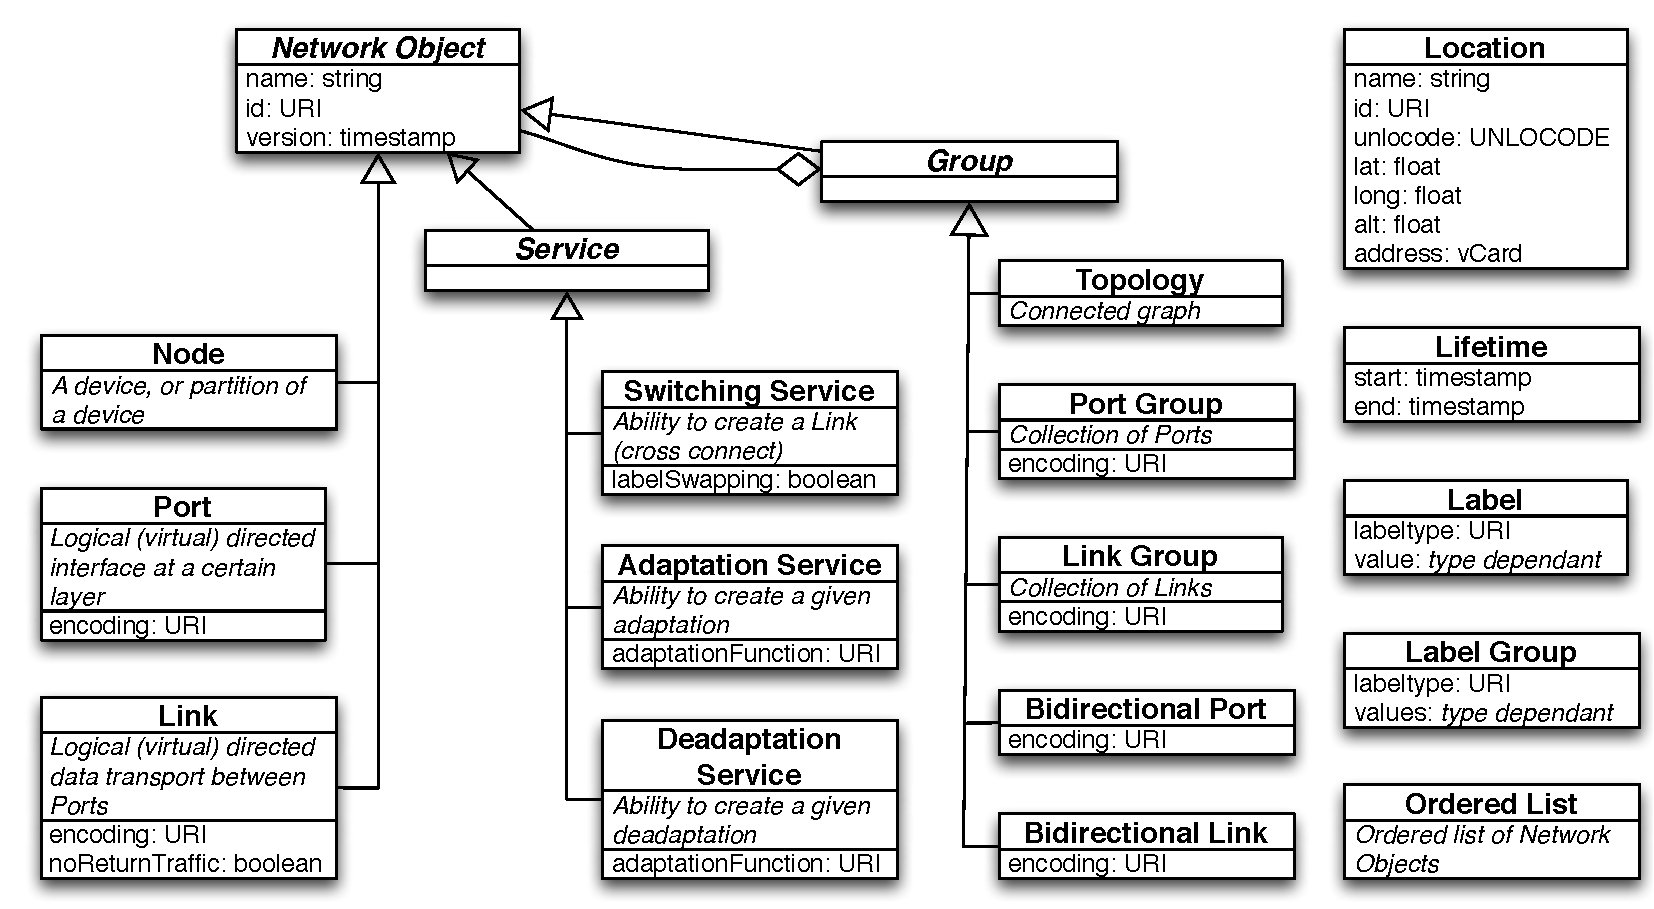
\includegraphics[width=\textwidth]{NML-hierarchy}
    \caption{A UML class diagram of the classes in the NML schema and their hierarchy}
    \label{fig:NML-schema}
\end{figure}

Figure~\ref{fig:NML-schema} shows an overview of all the classes in the NML schema in a UML class diagram. Each box defines the name of a class, a short description, and possible attributes with their value type.
%The figure also shows the relations between the objects, and their cardinalities. 
In the sections below we discuss each of the elements of the schema.

\subsubsection{Network Object}% (fold)
\label{class:network_object}

The basic abstract class of the schema is the \emph{Network Object}.  Most classes inherit from it.

\emph{Network Object} is an abstract class. It \MUSTNOT{} be instantiated directly.

A \emph{Network Object} may have the following relations:
\begin{itemize}
    \item \emph{existsDuring} to one or more \emph{Lifetime}s
    \item \emph{isAlias} to one or more \emph{Network Object}s
    \item \emph{locatedAt} to one \emph{Location} 
\end{itemize}

A \emph{Network Object} may have the following attributes:
\begin{itemize}
    \item \emph{id} to assign a persistent globally unique URI
    \item \emph{name} to assign a human readable string
    \item \emph{version} to assign a time stamp
\end{itemize}

The meaning of the \emph{isAlias} relation is only defined for specific cases (between objects of the same concrete class), and \SHOULDNOT{} be used between other objects.

The meaning of the \emph{version} attribute is only defined for specific cases (for objects of the Topology class), and \SHOULDNOT{} be used in other objects. Clients that receive a \emph{version} attribute for a non-\emph{Topology} object \SHOULD{} ignore that attribute.

An \emph{id} is a persistent, globally unique object identifier for the \emph{Network Object}. The \emph{id} \SHOULD{} be used to refer to this object. Section~\ref{s:identifiers} describes these identifiers in detail.

\emph{name} is a human readable string.
A name may be written in any language, but it is \RECOMMENDED{} that names are chosen so that all users can easily distinguish between different names. Names are not globally unique, and two objects can have the same name. It is \RECOMMENDED{} to use short, descriptive names.
A name \MUSTNOT{} be used for anything other than display purposes.  Normal Unicode recommendations apply: A name \MUSTNOT{} contain control or formatting codepoint, and it is \RECOMMENDED{} to only use codepoints from the Basic Multilingual Plane (BMP).

\emph{version} is a time stamp formatted as ISO 8601 calendar date, and \MUST{} be a basic (compact) representation with UTC timezone (\texttt{\emph{YYYYMMDD}T\emph{hhmmss}Z})~\cite{iso8601}. The time stamp can be used to publish updates of a \emph{Topology}. 
If a client receives multiple \emph{Topology} descriptions, each with a different version time stamp, the version with the latest time stamp in the past or present \MUST{} be considered the valid description. \emph{Topology} descriptions with a time stamp in the future \MAY{} be discarded or cached until the denoted time. See also the \emph{Lifetime} object to describe historic or future network changes.

The base \emph{Network Object} is subclassed into the top-level topology
components, that are sufficient to cover the description of networks.  The
classes in this schema that directly inherit from \emph{Network Object} are:

\begin{itemize}
    \item Node
    \item Port
    \item Link
    \item Service
    \item Group
\end{itemize}

These classes are described in more detail below.
% subsection network_object (end)


\subsubsection{Node}% (fold)
\label{class:node}

A \emph{Node} is generally a device connected to, or part of, the network.  A
Node does not necessarily correspond to a physical machine.

\emph{Node} inherits from \emph{Network Object}.

A \emph{Node} may have the following relations:
\begin{itemize}
    \item \emph{existsDuring} to one or more \emph{Lifetime}s
    \item \emph{hasInboundPort} to one or more \emph{Port}s or \emph{PortGroup}s
    \item \emph{hasOutboundPort} to one or more \emph{Port}s or \emph{PortGroup}s
    \item \emph{hasService} to one or more \emph{Service}s of type \emph{Switch}
    \item \emph{implementedBy} to one or more \emph{Node}s
    \item \emph{isAlias} to one or more \emph{Node}s
    \item \emph{locatedAt} to one \emph{Location} 
\end{itemize}

A \emph{Node} may have the following attributes:
\begin{itemize}
    \item \emph{id} to assign a persistent globally unique URI
    \item \emph{name} to assign a human readable string
\end{itemize}

% subsection node (end)


\subsubsection{Port}% (fold)
\label{class:port}

A \emph{Port} defines connectivity from a \emph{Network Object} to the rest of the network. A \emph{Port} object is unidirectional. A \emph{Port} does not necessarily correspond to a physical interface. It represents a logical transport entity at a fixed place in the network.

\emph{Port} inherits from \emph{Network Object}.

A \emph{Port} may have the following relations:
\begin{itemize}
    \item \emph{existsDuring} to one or more \emph{Lifetime}s
    \item \emph{hasLabel} to one \emph{Label}
    \item \emph{hasService} to one or more \emph{Service}s of type \emph{Adaptation} or type \emph{Deadaptation}
    \item \emph{isAlias} to one or more \emph{Port}s
    \item \emph{isSink} to one or more \emph{Link}s
    \item \emph{isSource} to one or more \emph{Link}s
\end{itemize}

A \emph{Port} may have the following attributes:
\begin{itemize}
    \item \emph{encoding} to assign a data encoding identifier
    \item \emph{id} to assign a persistent globally unique URI
    \item \emph{name} to assign a human readable string
\end{itemize}

The \emph{encoding} attribute defines the format of the data streaming through the Port. The identifier for the encoding \MUST{} be a URI. Encoding URIs \SHOULD{} be specified in a Grid Forum Documents (GFD).
% subsection port (end)


\subsubsection{Link}% (fold)
\label{class:link}

A \emph{Link} object describes a unidirectional data transport from each of its sources to all of its sinks.

A source of a Link is a Network Object, e.g.\ a \emph{Port}, that has a \emph{isSource} relation to the \emph{Link}.
A sink of a Link is a Network Object, e.g.\ a \emph{Port}, that has a \emph{isSink} relation to the \emph{Link}.

A \emph{Link} object can refer to any link connection. A link segment and an end-to-end path are both described by a \emph{Link} object. The composition of links into a path, and decomposition into link segments is described by the \emph{isSerialCompoundLink} relation.

\emph{Link} inherits from \emph{Network Object}.

A \emph{Link} may have the following relations:
\begin{itemize}
    \item \emph{existsDuring} to one or more \emph{Lifetime}s
    \item \emph{hasLabel} to one \emph{Label}
    \item \emph{isAlias} to one or more \emph{Link}s
    \item \emph{isSerialCompoundLink} to one \emph{Ordered List} of \emph{Link}s
\end{itemize}

A \emph{Link} may have the following attributes:
\begin{itemize}
    \item \emph{encoding} to assign a data encoding identifier
    \item \emph{id} to assign a persistent globally unique URI
    \item \emph{name} to assign a human readable string
\end{itemize}

A \emph{Link} may have the following parameter:
\begin{itemize}
    \item \emph{noReturnTraffic}. A value of \texttt{true} changes the definition of \emph{Link} to: data transport from each sources to all sinks, except that there is no data transport from a source to a sink if the source and sink are grouped together in a \emph{BidirectionalPort} group. The default value of \emph{noReturnTraffic} is \texttt{false}.
    
    An example of where this is used is in an Ethernet broadcast domain, where broadcast traffic is sent to all sinks, except the sink \emph{Port}s associated with the sending source \emph{Port}.
\end{itemize}

The \emph{encoding} attribute defines the format of the data streaming through the \emph{Link}. The identifier for the encoding \MUST{} be a URI. Encoding URIs \SHOULD{} be specified in a Grid Forum Documents (GFD).
% subsection link (end)


\subsubsection{Service}% (fold)
\label{class:service}

\emph{Service} describes an ability of the network. That is, it describes how the behavior can be changed dynamically.

\emph{Service} is an abstract class. It \MUSTNOT{} be instantiated directly.

\emph{Service} inherits from \emph{Network Object}.
A \emph{Service} may have the same relations, attributes and parameters as a \emph{Network Object}.

This schema defines three different services, the \emph{SwitchingService} the \emph{AdaptationService} and the \emph{DeadaptationService}. These are described in more detail below. 
% subsection service (end)


\subsubsection{Switching Service}% (fold)
\label{class:switching_service}

A \emph{SwitchingService} describes the ability to create new \emph{Link}s from any of its inbound \emph{Port}s to any of its outbound \emph{Port}s.

\emph{SwitchingService} inherits from \emph{Service}.

A \emph{SwitchingService} may have the following relations:
\begin{itemize}
    \item \emph{encoding} to assign a data encoding identifier
    \item \emph{existsDuring} to one or more \emph{Lifetime}s
    \item \emph{hasInboundPort} to one or more \emph{Port}s or \emph{PortGroup}s
    \item \emph{hasOutboundPort} to one or more \emph{Port}s or \emph{PortGroup}s
    \item \emph{isAlias} to one or more \emph{Switching Service}s
    \item \emph{providesLink} to one or more \emph{Link}s or \emph{LinkGroup}s.
\end{itemize}

A \emph{SwitchingService} may have the following attributes:
\begin{itemize}
    \item \emph{id} to assign a persistent globally unique URI
    \item \emph{name} to assign a human readable string
\end{itemize}

A \emph{SwitchingService} may have the following parameter:
\begin{itemize}
    \item \emph{labelSwapping}. A value of \texttt{false} adds a restriction to the \emph{SwitchingService}: it is only able to create cross connects from an inbound \emph{Port} to an outbound \emph{Port} if the \emph{Label} of the connected \emph{Port}s have the same value. The default value is \texttt{false}.
\end{itemize}

The \emph{providesLink} relation points to \emph{Link}s which describe the currently configured cross connects in a \emph{SwitchingService}.

A \emph{Port} object can have a \emph{hasService} relation, however the \emph{SwitchingService} defines a more specific relation \emph{hasInboundPort} / \emph{hasOutboundPort} relation to a \emph{Port} object. The latter relation is preferred over the \emph{hasService} relation of the Port to the SwitchingService.

The \emph{encoding} attribute defines the format of the data streaming through the \emph{SwitchingService}. The identifier for the encoding \MUST{} be a URI. Encoding URIs \SHOULD{} be specified in a Grid Forum Documents (GFD).
% subsection switching_service (end)


\subsubsection{Adaptation Service}% (fold)
\label{class:adaptation_service}

An \emph{AdaptationService} describes the ability that data from one or more \emph{Port}s can be embedded in the data encoding of one other \emph{Port}. This is commonly referred to as the embedding of client layer (higher network layer) ports in a server layer (lower network layer) port. The \emph{AdaptationService} describes a multiplexing adaptation function, meaning that different channels (the client layer ports) can be embedded in a single data stream (the server layer port). For example multiplexing several VLANs over a single trunk port.

Like \emph{Port} and \emph{Link}, \emph{AdaptationService} describes a unidirectional transport function. For the inverse transport function, see \emph{DeadaptationService}.

\emph{AdaptationService} inherits from \emph{Service}.

An \emph{AdaptationService} may have the following relations:
\begin{itemize}
    \item \emph{canProvidePort} to one or more \emph{Port}s or \emph{PortGroup}s (this describes a ability)
    \item \emph{existsDuring} to one or more \emph{Lifetime}s
    \item \emph{isAlias} to one or more \emph{AdaptationService}s
    \item \emph{providesPort} to one or more \emph{Port}s or \emph{PortGroup}s (this describes a configuration)
\end{itemize}

An \emph{AdaptationService} may have the following attributes:
\begin{itemize}
    \item \emph{adaptationFunction} to assign an adaptation technology identifier
    \item \emph{id} to assign a persistent globally unique URI
    \item \emph{name} to assign a human readable string
\end{itemize}

\emph{DeadaptationService} is an inverse of \emph{AdaptationService}. This should not be confused with an inverse multiplexing adaptation function. An inverse multiplexing adaptation function embeds a single data stream in multiple underlying data streams. To describes such a network, the \emph{parallelCompound} relation can be used, which is a future extension relation, described in a separate document~\cite{nml-experimental}.

% subsection adaptation_service (end)


\subsubsection{De-adaptation Service}% (fold)
\label{class:deadaptation_service}

A \emph{DeadaptationService} describes the ability that data of one or more ports can be extracted from the data encoding of one other port. This is commonly referred to as the extraction of client layer (higher network layer) ports from the server layer (lower network layer) port. The \emph{DeadaptationService} describes a demultiplexing adaptation function, meaning that different channels (the client layer ports) can be extracted from a single data stream (the server layer port). For example demultiplexing several VLANs from a single trunk port.

Like \emph{Port} and \emph{Link}, \emph{AdaptationService} describes a unidirectional transport function. For the inverse transport function, see \emph{AdaptationService}.%

\emph{DeadaptationService} inherits from \emph{Service}.

A \emph{DeadaptationService} may have the following relations:
\begin{itemize}
    \item \emph{canProvidePort} to one or more \emph{Port}s or \emph{PortGroup}s
    \item \emph{existsDuring} to one or more \emph{Lifetime}s
    \item \emph{isAlias} to one or more \emph{DeadaptationService}s
    \item \emph{providesPort} to one or more \emph{Port}s or \emph{PortGroup}s
\end{itemize}

A \emph{DeadaptationService} may have the following attributes:
\begin{itemize}
    \item \emph{adaptationFunction} to assign a adaptation technology identifier
    \item \emph{id} to assign a persistent globally unique URI
    \item \emph{name} to assign a human readable string
\end{itemize}

% subsubsection adaptation_service (end)


\subsubsection{Group}% (fold)
\label{class:group}

A \emph{Group} describes a collections of objects. Any object can be part of a group, including another \emph{Group}. An object can also be part of multiple \emph{Group}s.

\emph{Group} is an abstract class. It \MUSTNOT{} be instantiated directly.

\emph{Group} inherits from \emph{Network Object}.
A \emph{Group} may have the same relations, attributes and parameters as a \emph{Network Object}.

This schema defines five different \emph{Group}s:

\begin{itemize}
    \item Topology
    \item Port Group
    \item Link Group
    \item Bidirectional Port
    \item Bidirectional Link
\end{itemize}

These classes are described in more detail below.
% subsubsection group (end)



\subsubsection{Topology}% (fold)
\label{class:topology}

A \emph{Topology}\footnote{At first this was called a Network, then Graph Network. The term Topology was suggested to avoid the confusion surrounding the overloaded term Network.} is a set of connected \emph{Network Object}s. \emph{connected} means that there is, or it is possible to create, a data transport between any two Network Objects in the same Topology, provided that there are no policy, availability or technical restrictions.

A \emph{Topology} may have the following relations:
\begin{itemize}
    \item \emph{existsDuring} to one or more \emph{Lifetime}s
    \item \emph{hasNode} to one or more \emph{Node}s
    \item \emph{hasInboundPort} to one or more \emph{Port}s or \emph{PortGroup}s
    \item \emph{hasOutboundPort} to one or more \emph{Port}s or \emph{PortGroup}s
    \item \emph{hasService} to one or more \emph{Service} of type \emph{Switch}
    \item \emph{hasTopology} to one or more \emph{Topology}s
    \item \emph{isAlias} to one or more \emph{Topology}s
    \item \emph{locatedAt} to one \emph{Location} 
\end{itemize}

A \emph{Topology} may have the following attributes:
\begin{itemize}
    \item \emph{id} to assign a persistent globally unique URI
    \item \emph{name} to assign a human readable string
    \item \emph{version} to assign a serial number
\end{itemize}

The \emph{version} attribute is described at the \emph{Network Object}.
% subsubsection topology (end)


\subsubsection{Port Group}% (fold)
\label{class:port_group}

A \emph{PortGroup} is an unordered set of \emph{Port}s.

A \emph{PortGroup} may have the following relations:
\begin{itemize}
    \item \emph{existsDuring} to one or more \emph{Lifetime}s
    \item \emph{hasLabelGroup} to one \emph{LabelGroup}
    \item \emph{hasPort} to one or more \emph{Port}s or \emph{PortGroups}
    % \item \emph{hasService} to one or more \emph{Service}s of type Adaptation or type Deadaptation
    \item \emph{isAlias} to one or more \emph{PortGroup}s
    \item \emph{isSink} to one or more \emph{LinkGroup}s
    \item \emph{isSource} to one or more \emph{LinkGroup}s
\end{itemize}

A \emph{PortGroup} may have the following attributes:
\begin{itemize}
    \item \emph{encoding} to assign a data encoding identifier
    \item \emph{id} to assign a persistent globally unique URI
    \item \emph{name} to assign a human readable string
\end{itemize}

% subsubsection port_group (end)


\subsubsection{Link Group}% (fold)
\label{class:link_group}

A \emph{LinkGroup} is an unordered set of \emph{Link}s.

A \emph{LinkGroup} may have the following relations:
\begin{itemize}
    \item \emph{existsDuring} to one or more \emph{Lifetime}s
    \item \emph{hasLabelGroup} to one \emph{LabelGroup}
    \item \emph{hasLink} to one or more \emph{Link}s or \emph{LinkGroup}s
    \item \emph{isAlias} to one or more \emph{LinkGroup}s
    \item \emph{isSerialCompoundLink} to \emph{Ordered List} of \emph{LinkGroup}s
\end{itemize}

A \emph{LinkGroup} may have the following attributes:
\begin{itemize}
    \item \emph{id} to assign a persistent globally unique URI
    \item \emph{name} to assign a human readable string
\end{itemize}

% subsubsection link_group (end)


\subsubsection{Bidirectional Port}% (fold)
\label{class:bidirectional_port}

A \emph{BidirectionalPort} is a group of two (unidirectional) 
\emph{Port}s or \emph{PortGroup}s together forming a bidirectional representation of a physical or 
virtual port. See Figure~\ref{fig:Port-Link} for an example of a \emph{BidirectionalPort} and its associated \emph{Port}s.

A \emph{BidirectionalPort} may have the following relations:
\begin{itemize}
    \item \emph{existsDuring} to one or more \emph{Lifetime}s
    \item \emph{hasPort} to exactly two \emph{Port}s or two \emph{PortGroup}s
\end{itemize}

A \emph{BidirectionalPort} may have the following attributes:
\begin{itemize}
    \item \emph{encoding} to assign a data encoding identifier
    \item \emph{id} to assign a persistent globally unique URI
    \item \emph{name} to assign a human readable string
\end{itemize}

There is explicitly no direct relation between a \emph{BidirectionalPort} and a \emph{BidirectionalLink}, since NML is a unidirectional model.
% subsubsection bidirectional_port (end)

\begin{figure}[htbp]
    \centering
        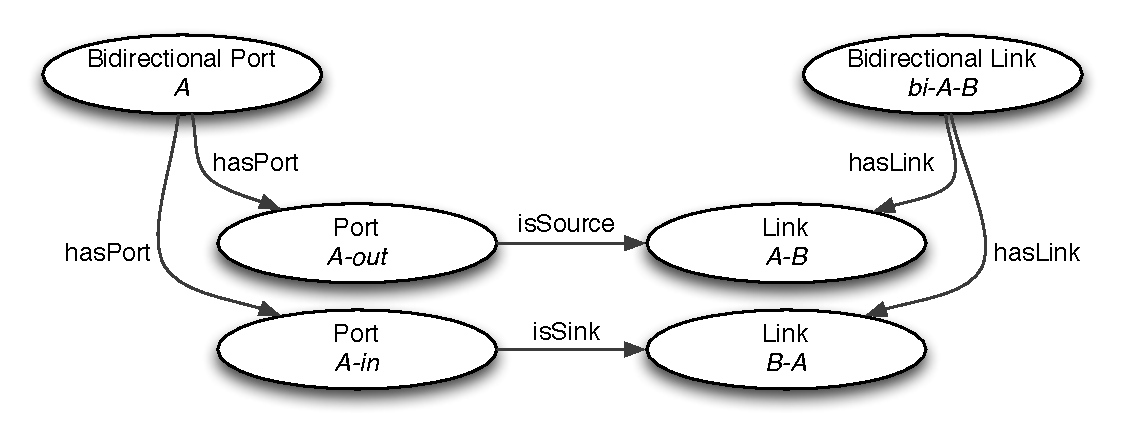
\includegraphics[width=.8\textwidth]{Port-Link.pdf}
    \caption{An abstract example of \emph{BidirectionalPort} and \emph{BidirectionalLink}}
    \label{fig:Port-Link}
\end{figure}


\subsubsection{Bidirectional Link}% (fold)
\label{class:bidirectional_link}

A \emph{BidirectionalLink} is a group of two (unidirectional) \emph{Link}s or \emph{LinkGroup}s together forming a bidirectional link. See Figure~\ref{fig:Port-Link} for an example of a \emph{BidirectionalLink} and its associated \emph{Link}s.

A \emph{BidirectionalLink} may have the following relations:
\begin{itemize}
    \item \emph{existsDuring} to one or more \emph{Lifetime}s
    \item \emph{hasLink} to exactly two \emph{Link}s or two \emph{LinkGroup}s
\end{itemize}

A \emph{BidirectionalLink} may have the following attributes:
\begin{itemize}
    \item \emph{encoding} to assign a data encoding identifier
    \item \emph{id} to assign a persistent globally unique URI
    \item \emph{name} to assign a human readable string
\end{itemize}

There is explicitly no direct relation between a \emph{BidirectionalPort} and a \emph{BidirectionalLink}, since NML is a unidirectional model.
% subsubsection bidirectional_link (end)


\subsubsection{Location}% (fold)
\label{class:location}

A \emph{Location} is a reference to a geographical location or area. A \emph{Location} object can be related to other \emph{Network Object}s to describe that these are located there. This can be relevant for network measurements, visualisations, et cetera.

A \emph{Location} may have the following attributes:
\begin{itemize}
    \item \emph{id} to assign a persistent globally unique URI
    \item \emph{name} to assign a human readable string
    \item \emph{long} is the longitude in WGS84 coordinate system (in decimal degrees)~\cite{wgs84}
    \item \emph{lat} is the latitude in WGS84 coordinate system (in decimal degrees)
    \item \emph{alt} is the altitude in WGS84 coordinate system (in decimal meters) 
    \item \emph{unlocode} is the UN/LOCODE location identifier~\cite{unlocode}
    \item \emph{address} is a vCard ADR (address) property. The exact syntax of the address property is not specified, to allow other (e.g.\ XML or RDF) representations of the string-based format specified in \cite{vcard}.
\end{itemize}

% subsubsection location (end)


\subsubsection{Lifetime}% (fold)
\label{class:lifetime}

A \emph{Lifetime} is an interval between which the object is said to be active. This can be used to track changes in a network, reflect dynamic operations, to help debug problems, et cetera.

A \emph{Lifetime} \MAY{} have the following attributes:
\begin{itemize}
    \item \emph{start} is the start time and date formatted as ISO 8601 calendar date, and \SHOULD{} be a basic (compact) representation with UTC timezone (\texttt{\emph{YYYYMMDD}T\emph{hhmmss}Z})~\cite{iso8601}
    \item \emph{end} is the end time and date formatted as ISO 8601 calendar date, and \SHOULD{} be a basic (compact) representation with UTC timezone (\texttt{\emph{YYYYMMDD}T\emph{hhmmss}Z})
\end{itemize}

Objects with multiple lifetimes mean that the lifetime of the object is the union of all lifetimes (as opposed to a intersection).

If a Network Object has no associated \emph{Lifetime} objects, or the start or end attribute of a Lifetime object is missing, the default lifetime may be assumed to start on or before the time specified in the version attribute of the most specific Topology object that contains this Network Object. The end of that assumed lifetime is indefinite, until a Topology object with a higher version number is published. This new description can define a new Lifetime for the object, or the Topology. If the new description does not contain the Network Object, the end time is assumed to have passed.

If a Network Object has no associated Lifetime objects, and the Topology object does not have a version attribute, than the lifetime of the Network Object is undefined.

% subsubsection lifetime (end)


\subsubsection{Label}% (fold)
\label{class:label}

A \emph{Label} is the technology-specific value that distinguishes a single data stream (a channel) embedded in a larger data stream. The \emph{Label} can be a resource label (with one value). In a future extension it may be a pair of source and destination labels (with two values)~\cite{g800}. Examples of resource labels are a VLAN number, wavelength, et cetera.

A \emph{Label} may have the following attributes:
\begin{itemize}
    \item \emph{labeltype} to refer to a technology-specific labelset, e.g.\ a URI for VLANs
    \item \emph{value} is one specific value taken from the labelset, e.g.\ a VLAN number
\end{itemize}

Technology extensions of NML may define additional attributes. Label type URIs \SHOULD{} be specified in a Grid Forum Documents (GFD), which \SHOULD{} also define possible values.

This version of NML only deals with resource labels. The use of source and destination labels is a future extension~\cite{nml-experimental}.


% subsubsection label (end)


\subsubsection{Label Group}% (fold)
\label{class:label_group}

A \emph{LabelGroup} is an unordered set of \emph{Label}s.

A \emph{LabelGroup} may have the following attributes:
\begin{itemize}
    \item \emph{labeltype} to refer to a technology-specific labelset
    \item \emph{values} is a set of specific values taken from the labelset
\end{itemize}

Technology extensions of NML may define additional attributes.
% subsubsection label_group (end)


\subsubsection{Ordered List}% (fold)
\label{class:ordered_list}

An \emph{Ordered List} is an ordered list of \emph{Network Object}s. These are used for the \emph{isSerialCompoundLink} relation to an ordered list of \emph{Link}s to describe a path through the network.

The representation of an \emph{Ordered List} depends on the syntax, and is defined in section~\ref{sub:ordered_lists}.
% subsubsection ordered_list (end)


\subsubsection{List Item}% (fold)
\label{class:list_item}

A \emph{ListItem} is a syntactical construct which may be used by syntaxes to construct a \emph{Ordered List}. The exact usage depends on the syntax.
% subsubsection list_item (end)



\subsection{Relations}
\label{sub:relations}

\emph{Relation}s describe how different \emph{Network Object}s relate to each other, 
typically to form a network topology description. 
The relations have been listed above, and are defined here (in alphabetical order). 
In principle a \emph{Relation} can go from any object to any other object. 

The list below makes a distinction between \emph{allowed} and \emph{defined} relations.
An \emph{allowed} relation means it is valid NML.
A \emph{defined} relation means that it has a specific meaning, as described here.

A relation which is \textsc{not} \emph{allowed} \MUST{} be rejected by a client, and the sender \SHOULD{} be notified with an error.
A relation which is \emph{allowed}, but (yet) \emph{undefined} \SHOULD{} be ignored by a client (either silently, or with a warning to the sender).
This distinction allows future extension of NML, while retaining limited backward compatibility.

The \emph{existsDuring}, \emph{hasLabel}, \emph{hasLabelGroup}, \emph{hasLink}, 
\emph{hasNode}, \emph{hasPort}, \emph{hasService}, \emph{hasTopology}, 
\emph{locatedAt}, \emph{providesLink}, and \emph{providesPort} are defined as 
\emph{implicit} relations. All other relations are \emph{explicit}. 
The distinction between implicit and explicit relations may be used by a syntax to 
allow a more compact network description.

\subsubsection{canProvidePort}% (fold)
\label{rel:canProvidePort}

\emph{canProvidePort} is used to relate an \emph{AdaptationService} or 
\emph{DeadaptationService} to one or more \emph{Port}s or \emph{PortGroup}s 
to define that these can be created by that \emph{AdaptationService} or 
\emph{DeadaptationService}.

Allowed relations are:
\begin{itemize}
    \item \nmlrelation{Service}{*}{canProvidePort}{*}{Port}
    \item \nmlrelation{Service}{*}{canProvidePort}{*}{PortGroup}
\end{itemize}

Defined relations are:
\begin{itemize}
    \item \nmlrelation{AdaptationService}{*}{canProvidePort}{*}{Port}
    \item \nmlrelation{AdaptationService}{*}{canProvidePort}{*}{PortGroup}
    \item \nmlrelation{DeadaptationService}{*}{canProvidePort}{*}{Port}
    \item \nmlrelation{DeadaptationService}{*}{canProvidePort}{*}{PortGroup}
\end{itemize}

\subsubsection{existsDuring}% (fold)
\label{rel:existsDuring}

\emph{existsDuring} relates one \emph{Network Object} object to zero or more \emph{LifeTime} objects. This defines the existence of the object at a certain time.

\nmlrelation{Network Object}{1}{existsDuring}{*}{LifeTime}

Objects with multiple lifetimes mean that the lifetime of the object is the union of all lifetimes (as opposed to a intersection).

If a Network Object has no associated Lifetime objects, or the start or end attribute of a Lifetime object is missing, the default lifetime may be assumed to start on or before the time specified in the version attribute of the most specific Topology object that contains this Network Object, and the end on or later than the version attribute of the next published Topology object.

If a Network Object has no associated Lifetime objects, and the Topology object does not have a version attribute, then the lifetime of the Network Object is undefined.

\subsubsection{hasInboundPort}% (fold)
\label{rel:hasInboundPort}

\emph{hasInboundPort} defines the relation between a \emph{Node}, a \emph{SwitchingService} or a \emph{Topology} and their respective \emph{Port}s or \emph{PortGroup}s

Allowed relations are:
\begin{itemize}
    \item \nmlrelation{Network Object}{*}{hasInboundPort}{*}{Port}
    \item \nmlrelation{Network Object}{*}{hasInboundPort}{*}{PortGroup}
\end{itemize}

Defined relations are:
\begin{itemize}
    \item \nmlrelation{Node}{*}{hasInboundPort}{*}{Port}
    \item \nmlrelation{Node}{*}{hasInboundPort}{*}{PortGroup}
    \item \nmlrelation{SwitchingService}{*}{hasInboundPort}{*}{Port}
    \item \nmlrelation{SwitchingService}{*}{hasInboundPort}{*}{PortGroup}
    \item \nmlrelation{Topology}{*}{hasInboundPort}{*}{Port}
    \item \nmlrelation{Topology}{*}{hasInboundPort}{*}{PortGroup}
\end{itemize}

This defines that the related \emph{Network Object} has an inbound \emph{Port} or \emph{PortGroup} object. The direction of the \emph{Port} object is relative to the \emph{Network Object} the \emph{Port} is attached to, so in this case the traffic flows towards that \emph{Network Object} (similarly for the \emph{PortGroup}). This \emph{Port} would then be related to a \emph{Link} object using the \emph{isSink} relation (or a \emph{PortGroup} and \emph{LinkGroup} respectively).

A \emph{Network Object} with a \emph{hasInboundPort} relation pointing to a \emph{PortGroup} has the same meaning as defining a \emph{hasInboundPort} relation pointing to every \emph{Port} in that \emph{PortGroup} (as defined by a \emph{hasPort} relation between the \emph{PortGroup} and \emph{Port}).


\subsubsection{hasLabel}% (fold)
\label{rel:hasLabel}

\emph{hasLabel} assigns one \emph{Label} to a \emph{Port} or \emph{Link}

Allowed relations are:
\begin{itemize}
    \item \nmlrelation{Port}{1}{hasLabel}{*}{Label}
    \item \nmlrelation{Link}{1}{hasLabel}{*}{Label}
\end{itemize}

The \emph{Label} assigned to a \emph{Port} or \emph{Link} is the technology label that identifies the traffic through this \emph{Port} or \emph{Link} (including in \emph{Link}s provided by a \emph{SwitchingMatrix}).

A \emph{Label} is used to distinguish a \emph{Port} in a \emph{PortGroup}, or distinguish a \emph{Link} in a \emph{LinkGroup}.

The meaning of \emph{hasLabel} is only \emph{defined} for a cardinality of 0 or 1.


\subsubsection{hasLabelGroup}% (fold)
\label{rel:hasLabelGroup}

\emph{hasLabelGroup} assigns one \emph{LabelGroup} to a \emph{PortGroup} or \emph{LinkGroup}

Allowed relations are:
\begin{itemize}
    \item \nmlrelation{PortGroup}{1}{hasLabelGroup}{*}{LabelGroup}
    \item \nmlrelation{LinkGroup}{1}{hasLabelGroup}{*}{LabelGroup}
\end{itemize}

The \emph{LabelGroup} assigned to this \emph{PortGroup} or \emph{LinkGroup} defines the \emph{Label}s associated with the \emph{Port}s member of that group. There  \MUST{} be a one-to-one correspondence between the \emph{LabelGroup} and the \emph{PortGroup}.

The meaning of \emph{hasLabelGroup} is only defined for a cardinality of 0 or 1.

\subsubsection{hasLink}% (fold)
\label{rel:hasLink}

\emph{hasLink} is used for:
    \begin{itemize}
        \item \emph{BidirectionalLink} to relate exactly two \emph{Link}s or two \emph{LinkGroup}s
        \item \emph{LinkGroup} to one or more \emph{Link}s or \emph{LinkGroup}s to define membership of that group
    \end{itemize}

Allowed relations are:
\begin{itemize}
    \item \nmlrelation{Group}{*}{hasLink}{*}{Link}
    \item \nmlrelation{Group}{*}{hasLink}{*}{LinkGroup}
\end{itemize}

Defined relations are:
\begin{itemize}
    \item \nmlrelation{LinkGroup}{*}{hasLink}{*}{Link}
    \item \nmlrelation{LinkGroup}{*}{hasLink}{*}{LinkGroup}
    \item \nmlrelation{BidirectionalLink}{*}{hasLink}{2}{Link}
    \item \nmlrelation{BidirectionalLink}{*}{hasLink}{2}{LinkGroup}
\end{itemize}

The \emph{hasLink} relationships for a \emph{BidirectionalLink} point to the two unidirectional \emph{Link}s that together form a bidirectional connection between its respective associated \emph{Node}s.

The \emph{hasLink} relationships for a \emph{LinkGroup} define the membership of the \emph{Link}s in that \emph{LinkGroup}.

\subsubsection{hasNode}% (fold)
\label{rel:hasNode}

\emph{hasNode} relates a \emph{Topology} to a \emph{Node}, meaning that a \emph{Node} is part of a \emph{Topology}

Allowed relations are:
\begin{itemize}
    \item \nmlrelation{Network Object}{*}{hasNode}{*}{Node}
\end{itemize}

Defined relations are:
\begin{itemize}
    \item \nmlrelation{Topology}{*}{hasNode}{*}{Node}
\end{itemize}


\subsubsection{hasOutboundPort}% (fold)
\label{rel:hasOutboundPort}

\emph{hasOutboundPort} relates either a \emph{Node}, \emph{SwitchingService} or a \emph{Topology} to one or more \emph{Port}s or \emph{PortGroup}s.

Allowed relations are:
\begin{itemize}
    \item \nmlrelation{Network Object}{*}{hasOutboundPort}{*}{Port}
    \item \nmlrelation{Network Object}{*}{hasOutboundPort}{*}{PortGroup}
\end{itemize}

Defined relations are:
\begin{itemize}
    \item \nmlrelation{Node}{*}{hasOutboundPort}{*}{Port}
    \item \nmlrelation{Node}{*}{hasOutboundPort}{*}{PortGroup}
    \item \nmlrelation{SwitchingService}{*}{hasOutboundPort}{*}{Port}
    \item \nmlrelation{SwitchingService}{*}{hasOutboundPort}{*}{PortGroup}
    \item \nmlrelation{Topology}{*}{hasOutboundPort}{*}{Port}
    \item \nmlrelation{Topology}{*}{hasOutboundPort}{*}{PortGroup}
\end{itemize}

This defines that the related \emph{Network Object} has an outbound \emph{Port} or \emph{PortGroup} object. The direction of the \emph{Port} object is relative to the \emph{Network Object} the \emph{Port} is attached to, so in this case the traffic flows away from that \emph{Network Object} (similarly for the \emph{PortGroup}). This \emph{Port} would then be related to a \emph{Link} object using the \emph{isSource} relation (or az \emph{PortGroup} and \emph{LinkGroup} respectively).

A \emph{Network Object} with a \emph{hasOutboundPort} relation pointing to a \emph{PortGroup} has the same meaning as defining a \emph{hasOutboundPort} relation pointing to every \emph{Port} in that \emph{PortGroup} (as defined by a \emph{hasPort} relation between the \emph{PortGroup} and \emph{Port}).

\subsubsection{hasPort}% (fold)
\label{rel:hasPort}

\emph{hasPort} is used for:
    \begin{itemize}
        \item \emph{BidirectionalPort} to relate exactly two \emph{Port}s or two \emph{PortGroup}s
        \item \emph{PortGroup} to one or more \emph{Port}s or \emph{PortGroup}s
    \end{itemize}

Allowed relations are:
\begin{itemize}
    \item \nmlrelation{Group}{*}{hasPort}{*}{Port}
    \item \nmlrelation{Group}{*}{hasPort}{*}{PortGroup}
\end{itemize}

Defined relations are:
\begin{itemize}
    \item \nmlrelation{PortGroup}{*}{hasPort}{*}{Port}
    \item \nmlrelation{PortGroup}{*}{hasPort}{*}{PortGroup}
    \item \nmlrelation{BidirectionalPort}{*}{hasPort}{2}{Port}
    \item \nmlrelation{BidirectionalPort}{*}{hasPort}{2}{PortGroup}
\end{itemize}

The \emph{hasPort} relationships for a \emph{BidirectionalPort} point to the two unidirectional \emph{Port}s that together form a bidirectional port for the associated \emph{Node}. These \emph{Port}s would have a \emph{hasInboundPort} and \emph{hasOutboundPort} relation with that \emph{Node}.

The \emph{hasPort} relationships for a \emph{PortGroup} define the membership of the \emph{Port}s in that \emph{PortGroup}.

\subsubsection{hasService}% (fold)
\label{rel:hasService}

\emph{hasService} relates a \emph{Network Object} to a \emph{Service}. This schema only defines the meaning of:
    \begin{itemize}
        \item \emph{Port} to \emph{AdaptationService}, relating one server-layer \emph{Port} to an adaptation function.
        \item \emph{Port} to \emph{DeadaptationService}, relating one server-layer \emph{Port} to a deadaptation function.
        \item \emph{Node} or \emph{Topology} to \emph{SwitchingService}, describing a switching ability of that \emph{Node} or \emph{Topology}.
    \end{itemize}

Allowed relations are:
\begin{itemize}
    \item \nmlrelation{Network Object}{*}{hasService}{*}{Service}
\end{itemize}

Defined relations are:
\begin{itemize}
    \item \nmlrelation{Port}{1}{hasService}{*}{AdaptationService}
    \item \nmlrelation{Port}{1}{hasService}{*}{DeadaptationService}
    \item \nmlrelation{Node}{*}{hasService}{*}{SwitchingService}
    \item \nmlrelation{Topology}{*}{hasService}{*}{SwitchingService}
\end{itemize}

A \emph{Port} object can have a \emph{hasService} relation to a \emph{Service}, however the \emph{SwitchingService} defines a more specific relation \emph{hasInboundPort} / \emph{hasOutboundPort} relation to a \emph{Port} object. The latter relation is preferred over the \emph{hasService} relation of the \emph{Port} to the \emph{SwitchingService}.


\subsubsection{hasTopology}% (fold)
\label{rel:hasTopology}

\emph{hasTopology} defines a relation between one \emph{Topology} to one or more \emph{Topology}s for aggregation purposes.

Allowed relations are:
\begin{itemize}
    \item \nmlrelation{Network Object}{*}{hasTopology}{*}{Topology}
\end{itemize}


Defined relations are:
\begin{itemize}
    \item \nmlrelation{Topology}{*}{hasTopology}{*}{Topology}
\end{itemize}


\subsubsection{implementedBy}% (fold)
\label{rel:implementedBy}

\emph{implementedBy} relates a \emph{Node} to one or more \emph{Node}s to describe virtualization or partitioning of a \emph{Node}. 
The relation \MAY{} be recursive, thus a virtual \emph{Node} \MAY{} be further partitioned.

Allowed relations are:
\begin{itemize}
    \item \nmlrelation{Network Object}{*}{implementedBy}{*}{Network Object}
\end{itemize}

Defined relations are:
\begin{itemize}
    \item \nmlrelation{Node}{*}{implementedBy}{*}{Node}
\end{itemize}

\subsubsection{isAlias}% (fold)
\label{rel:isAlias}

\emph{isAlias} is a relation from a \emph{Network Object} to a \emph{Network Object} to describe that one can be used as the alias of another.

Allowed relations are:
\begin{itemize}
    \item \nmlrelation{Network Object}{*}{isAlias}{*}{Network Object}
\end{itemize}

The relation is only defined if the type of both objects is the same (e.g.\ a Node can be related to another Node, but if it is related to a Topology using the \emph{isAlias} relation, that relation is \emph{undefined}.)

% NOTE: We currently /allow/ isAlias between different type of network objects,
% although it is /undefined/ (meaning: it is not an error, 
% only a warning, and may be defined in the future.)
% I can't imagine we want this in the future, so /not allowed/ seems preferred.
% The main reason for not changing this is that there is no way to codify this
% into the RDF and OWL schemas. [FD]


\subsubsection{isSerialCompoundLink}% (fold)
\label{rel:isSerialCompoundLink}

\emph{isSerialCompoundLink} is used to define that a \emph{Link} or \emph{LinkGroup} represents an \emph{Ordered List} of \emph{Link}s or \emph{LinkGroup}s. This must include cross-connects.

The following relation is allowed and defined:
\begin{itemize}
    \item \nmlrelation{Link}{1}{isSerialCompoundLink}{*}{\lower4ex\vbox{\hbox{1. \framebox{Link}}\hbox{2. \framebox{Link}}\hbox{\hspace{2em}...}\hbox{n. \framebox{Link}}}}
\end{itemize}

The following relation is allowed, but undefined:
\begin{itemize}
    \item \nmlrelation{LinkGroup}{*}{isSerialCompoundLink}{*}{\lower4ex\vbox{\hbox{1. \framebox{LinkGroup}}\hbox{2. \framebox{LinkGroup}}\hbox{\hspace{3.4em}...}\hbox{n. \framebox{LinkGroup}}}}
\end{itemize}


\subsubsection{isSink}% (fold)
\label{rel:isSink}

\emph{isSink} relates a \emph{Port} to one \emph{Link} to define the outgoing traffic port, and similarly for \emph{PortGroup} and \emph{LinkGroup}.

Allowed relations are:
\begin{itemize}
    \item \nmlrelation{Network Object}{*}{isSink}{*}{Link}
    \item \nmlrelation{Network Object}{*}{isSink}{*}{LinkGroup}
\end{itemize}

Defined relations are:
\begin{itemize}
    \item \nmlrelation{Port}{*}{isSink}{*}{Link}
    \item \nmlrelation{PortGroup}{*}{isSink}{*}{LinkGroup}
\end{itemize}

\emph{isSink} between a \emph{PortGroups} and a \emph{LinkGroup} is \emph{defined} only if the \emph{PortGroup} and \emph{LinkGroup} in question have the exact same \emph{LabelGroup}.


\subsubsection{isSource}% (fold)
\label{rel:isSource}

\emph{isSource} relates a \emph{Port} to one \emph{Link} to define its incoming traffic port, and similarly for \emph{PortGroup} and \emph{LinkGroup}.

Allowed relations are:
\begin{itemize}
    \item \nmlrelation{Network Object}{*}{isSource}{*}{Link}
    \item \nmlrelation{Network Object}{*}{isSource}{*}{LinkGroup}
\end{itemize}

Defined relations are:
\begin{itemize}
    \item \nmlrelation{Port}{*}{isSource}{*}{Link}
    \item \nmlrelation{PortGroup}{*}{isSource}{*}{LinkGroup}
\end{itemize}

\emph{isSource} between a \emph{PortGroups} and a \emph{LinkGroup} is \emph{defined} only if the \emph{PortGroup} and \emph{LinkGroup} in question have the exact same \emph{LabelGroup}.


\subsubsection{item}% (fold)
\label{class:item}

A \emph{item} relation is a syntactical construct which may be used by syntaxes to construct a \emph{Ordered List}. The exact usage depends on the syntax.
% subsubsection item (end)


\subsubsection{locatedAt}% (fold)
\label{rel:locatedAt}

\emph{locatedAt} relates a \emph{Network Object} to one \emph{Location} to describe that a \emph{Network Object} is located at that \emph{Location}.

\begin{itemize}
    \item \nmlrelation{Network Object}{*}{locatedAt}{*}{Location}
\end{itemize}


\subsubsection{next}% (fold)
\label{rel:next}

\emph{next} relation is a syntactical construct which may be used by syntaxes to construct a \emph{Ordered List}. The exact usage depends on the syntax.
% subsubsection next (end)


\subsubsection{providesLink}% (fold)
\label{rel:providesLink}

\emph{providesLink} is used to relate a \emph{SwitchingService} to one or more \emph{Link}s or \emph{LinkGroup}s to define that these have been created by that \emph{SwitchingService}.

Allowed relations are:
\begin{itemize}
    \item \nmlrelation{Service}{*}{providesLink}{*}{Link}
    \item \nmlrelation{Service}{*}{providesLink}{*}{LinkGroup}
\end{itemize}

Defined relations are:
\begin{itemize}
    \item \nmlrelation{SwitchingService}{1}{providesLink}{*}{Link}
    \item \nmlrelation{SwitchingService}{1}{providesLink}{*}{LinkGroup}
\end{itemize}


\subsubsection{providesPort}% (fold)
\label{rel:providesPort}

\emph{providesPort} is used to relate an \emph{AdaptationService} or \emph{DeadaptationService} to one or more \emph{Port}s or \emph{PortGroup}s to define that these have been created by that \emph{AdaptationService} or \emph{DeadaptationService}.

Allowed relations are:
\begin{itemize}
    \item \nmlrelation{Service}{*}{providesPort}{*}{Port}
    \item \nmlrelation{Service}{*}{providesPort}{*}{PortGroup}
\end{itemize}

Defined relations are:
\begin{itemize}
    \item \nmlrelation{AdaptationService}{1}{providesPort}{*}{Port}
    \item \nmlrelation{AdaptationService}{1}{providesPort}{*}{PortGroup}
    \item \nmlrelation{DeadaptationService}{1}{providesPort}{*}{Port}
    \item \nmlrelation{DeadaptationService}{1}{providesPort}{*}{PortGroup}
\end{itemize}


\subsection{Attributes}
\label{sub:attributes}

\emph{Attributes} are properties of an object. The following attributes have been defined in section~\ref{sub:classes}.

\begin{tabular}{@{}p{0.25\textwidth}p{0.72\textwidth}}
\textbf{Attribute} &                                                                                   \textbf{Class (section)}\\
adaptationFunction & AdaptationService (\ref{class:adaptation_service}), DeadaptationService (\ref{class:deadaptation_service})\\
           address &                                                                            Location (\ref{class:location})\\
               alt &                                                                            Location (\ref{class:location})\\
          encoding & Port (\ref{class:port}), Link (\ref{class:link}), PortGroup (\ref{class:port_group}), LinkGroup (\ref{class:link_group}), BidirectionalPort (\ref{class:bidirectional_link}), BidirectionalLink (\ref{class:bidirectional_link}),SwitchingService (\ref{class:switching_service})\\
               end &                                                                            LifeTime (\ref{class:lifetime})\\
                id &                                NetworkObject (\ref{class:network_object}), Location (\ref{class:location})\\
         labeltype &                                            Label (\ref{class:label}), LabelGroup (\ref{class:label_group})\\
               lat &                                                                            Location (\ref{class:location})\\
              long &                                                                            Location (\ref{class:location})\\
              name &                                                             NetworkObject, Location (\ref{class:location})\\
             start &                                                                            LifeTime (\ref{class:lifetime})\\
          unlocode &                                                                            Location (\ref{class:location})\\
             value &                                                                                  Label (\ref{class:label})\\
            values &                                                                       LabelGroup (\ref{class:label_group})\\
           version &                                                                 NetworkObject (\ref{class:network_object})\\
\end{tabular}


\subsection{Parameters}
\label{sub:parameters}

\emph{Parameters} are properties of an object.
Parameters, like attributes, are properties of objects, but may (subtly) change 
the logic of the object.
The following parameters have been defined in section~\ref{sub:classes}.

\begin{tabular}{@{}p{0.25\textwidth}p{0.72\textwidth}}
\textbf{Parameter} &                         \textbf{Class (section)}\\
     labelSwapping & SwitchingService (\ref{class:switching_service})\\
   noReturnTraffic &                          Link (\ref{class:link})\\

\end{tabular}


%!TEX root = nml-base.tex

\section{Identifiers}%
\label{s:identifiers}

\subsection{Schema Identifier}%
\label{sub:schema_uri}

% The \path command is from the hyperref package, it is the non-clickable variant of the \url command. It does do nice wrapping for URLs/paths/etc.
The namespace for the schema defined in document is \path{http://schemas.ogf.org/nml/2013/05/base\#}.

All classes, relations, parameters and attributes defined in this document reside in this namespace. For example, the Link class is identified by \texttt{http://schemas.ogf.org/nml/2013/05/base\#Link}

\subsection{Instance Identifiers}%
\label{sub:identifiers}

Section \ref{class:network_object} requires that instances of Network Objects \SHOULD{} have an \emph{id} attribute, which \MUST{} be a unique URI.

% It is possible to describe additional information on an instance, in this case an \emph{idRef} attribute can be used.

Implementations that receive a network topology description \MUST{} be prepared to accept any valid URI as an identifier.

Implementations that publish a network topology description instance identifiers \MAY{} adhere to the syntax of Global Network Identifiers as defined in~\cite{gfd-urn-ogf-network}, which ensures global uniqueness and easy recognition as Network Object instances.

Two different Network Objects instances \MUST{} have two different identifiers.

Once an identifier is assigned to a resource, it \MUSTNOT{} be re-assigned to another resource.

A URI \MAY{} be interpreted as an International Resource Identifier (IRI) for display purposes, but URIs from external source domains \MUSTNOT{} be IRI-normalised before transmitting to others.

\subsubsection{Lexical Equivalence}

Two identifier are lexical equivalent if they are binary equivalent after case folding\footnote{\emph{Case folding} is primarily used for caseless comparison of text. \emph{Case mapping} is used for display purposes.}~\cite{casefolding}.

Other interpretation (such as percent-decoding or Punycode decoding~\cite{punycode}) \MUSTNOT{} take place.

For the purpose of equivalence comparison, any possible fragment part or query part of the URI is considered part of the URI.

For example the following identifiers are equivalent:

\begin{quote}
  \texttt{1 - urn:ogf:network:example.net:2013:local\_string\_1234}\\
  \texttt{2 - URN:OGF:network:EXAMPLE.NET:2013:Local\_String\_1234}
\end{quote}

While the following identifiers are not equivalent (in this case, the percentage encoding even makes URI \#3 an invalid Global Network Identifier.):

\begin{quote}
  \texttt{1 - urn:ogf:network:example.net:2013:local\_string\_1234}\\
  \texttt{3 - urn:ogf:network:example.net:2013:local\%5Fstring\%5F1234}
\end{quote}

\subsubsection{Further Restrictions}

An assigning organisation \MUSTNOT{} assign Network Object Identifier longer than 255 characters in length.

Parsers \MUST{} be prepared to accept identifiers of up to 255 characters in length.

A Parser \SHOULD{} verify if an identifier adheres to the general URI syntax rules, as specified in RFC 3986~\cite{rfc3986}.

Parsers \SHOULD{} reject identifiers which do not adhere to the specified rules. A parser encountering an invalid identifier \SHOULD{} reply with an error code that includes the malformed identifier, but \MAY{} accept the rest of the message, after purging all references to the Network Object with the malformed identifier.

\subsubsection{Interpreting Identifiers}

A Network Object identifier \MUST{} be treated as a opaque string, only used to uniquely identify a Network Object. The local-part of a Global Network Identifier \MAY{} have certain meaning to it's assigning organisation, but \MUSTNOT{} be interpreted by any other organisation.

\subsubsection{Network Object Attribute Change}

A Network Object may change during its lifetime. If these changes are so drastic that the assigning organisation considers it a completely new Network Object, the assigning organisation should be assigned a new identifier. In this case, other organisations MUST treat this object as completely new Network Resource.

If the assigning organisation considers the changes are small, it \MUST{} retain the same identifier for the Network Object, and use some mechanism to signal it's peers of the changes in the attributes of the Network Object. An appropriate mechanism is to send a new description of the Topology or the Network Object with an updated \emph{version} attribute.

\subsection{Unnamed Objects}%
\label{sub:unnamed_objects}

Network Objects that do not have a regular URI as id attribute, may have either:
\begin{itemize}
    \item Have no id attribute. These are so-called \emph{unnamed} network objects.
    \item Have an id attribute which is a fragment identifier only, thus an URI starting with a crosshatch (\texttt{\#}) character. These are so-called \emph{ad-hoc named} network objects.
\end{itemize}

A \emph{unnamed} network object can not be referenced. A network objects generally \SHOULDNOT{} be unnamed, since there is no possibility for an external party to refer to the object.

A \emph{ad-hoc named} network object can only be referenced from within the same topology description. \emph{ad-hoc} \emph{id}s must be considered a syntactical construct, not as a persistent identifier. The \MUSTNOT{} be referred to from another scope or another topology description. \emph{ad-hoc id}s \SHOULDNOT{} be stored. If a two peers exchange topology messages, it is perfectly valid to change the ad-hoc id in each message (since they are only valid within scope of that message anyway).

A possible reason to use unnamed or ad-hoc named network objects it to make a statement such as \textit{“Port A and Port B are grouped in a BidirectionalPort”} without actually assigning an identifier to this BidirectionalPort.




%!TEX root = nml-base.tex

\section{Syntax}
\label{s:syntax}

The Network Markup Language has two different normative syntaxes. The syntaxes are in regular XML defined using an XML Schema (XSD), and another in OWL RDF/XML syntax, defined in an OWL schema.
The OWL syntax is aimed at Semantic Web-oriented applications, the XML syntax is suitable for any application. These syntaxes are defined in Appendices \ref{s:xmlschema} and \ref{s:owlschema} respectively. These syntaxes follow the model as defined in section~\ref{s:schema}, should there be any inconsistencies between the syntaxes or the syntaxes and the model, the definitions in section~\ref{s:schema} take precedence.


\subsection{XML Syntax} % (fold)
\label{sub:xml}

An NML object is represented as an XML element. For example:
\begin{lstlisting}
<nml:BidirectionalLink />
\end{lstlisting}

An NML attribute or parameter is represented as either an XML attribute, XML child element or text value of the XML element. The table list the mapping for the attributes and parameters defined in this document:

\begin{tabular}{|l|c|c|c|}
\hline
\textbf{XML representation} & \textbf{Attribute} & \textbf{Child element} & \textbf{Text of element} \\
\hline
\textbf{NML attribute or parameter} & id & name & value \\
 & adaptationFunction & address & values \\
 & encoding & lat & \\
 & labeltype & long & \\
 & version & alt & \\
 & noReturnTraffic & unlocode & \\
 & labelSwapping & start & \\
 &  & end & \\
% \hline
% \textbf{XML representation} & \textbf{Attribute} & \textbf{Child element} & \textbf{Text of element} \\
\hline
\end{tabular}

For example:
\begin{lstlisting}
<nml:Port id="urn:ogf:network:example.net:2013:port_X.1501:in">
  <nml:name>VLAN 1501 at Port X (in)</nml:name>
  <nml:Label labeltype="http://schemas.ogf.org/nml/2013/05/ethernet#vlan">1501</nml:Label>
</nml:Port>
\end{lstlisting}

Explicit relation are represented as a \texttt{<nml:Relation>} XML element, with the domain as the parent element, and the range as the child element. Implicit relations are not given: the range object is represented as an XML child element of the domain. 
Below is an example of an explicit relation:
\begin{lstlisting}
<nml:Port id="urn:ogf:network:example.net:2013:port_X:in">
  <nml:Relation type="http://schemas.ogf.org/nml/2013/05/base#isSource">
    <nml:Link id="urn:ogf:network:example.net:2013:linkA:XY"/>
  </nml:Relation>
</nml:Port>
\end{lstlisting}
And this is an example of an implicit relation:
\begin{lstlisting}
<nml:Topology id="urn:ogf:network:example.net:2013:Example_Network">
  <nml:Node id="urn:ogf:network:example.net:2013:example_node"/>
</nml:Port>
\end{lstlisting}

% subsection xml (end)




\subsection{OWL RDF/XML Syntax} % (fold)
\label{sub:owl}

An NML object is represented as an RDF subject. Exceptions are \emph{Label} and \emph{LabelGroup}.

An NML attribute or parameter is represented as a predicate. 

For example:
\begin{lstlisting}
<nml:Location id="urn:ogf:network:example.net:2013:redcity">
  <nml:name>Red City</nml:name>
  <nml:lat>30.600</nml:lat>
  <nml:long>12.640</nml:long>
</nml:Location>
\end{lstlisting}

Relations are represented as an RDF triplet, with the full URI of the attribute or parameter.  For example:
\begin{lstlisting}
<nml:Port rdf:about="urn:ogf:network:example.net:2013:port_X:in">
   <nml:isSource rdf:resource="urn:ogf:network:example.net:2013:linkA:XY"/>
</nml:Port>
\end{lstlisting}

A \emph{Label} is represented as a two triplets: one triplet defining a labeltype as a subproperty of the abstract Label resource, and one relating a Port or Link to a value using this labeltype.  For example:

\begin{lstlisting}
<rdf:Description rdf:about="http://schemas.ogf.org/nml/2013/05/ethernet#vlan">
  <owl:subPropertyOf rdf:resource="http://schemas.ogf.org/nml/2013/05/base#hasLabel"/>
</rdf:Description>
<nml:Port rdf:about="urn:ogf:network:example.net:2013:port_X.1501:in">
  <nmleth:vlan>1501</nmleth:vlan>
</nml:Port>
\end{lstlisting}

A \emph{LabelGroup} is represented as three triplets. The URI of the labeltype is not the URI of the predicate, to avoid naming clashes with the definition of the Label. Instead, the predicate of the LabelGroup is related to the predicate of the Label using the nml:labeltype property:
\begin{lstlisting}
<rdf:Description rdf:about="http://schemas.ogf.org/nml/2013/05/ethernet#vlans">
  <nml:labelType rdf:resource="http://schemas.ogf.org/nml/2013/05/ethernet#vlan"/>
  <owl:subPropertyOf rdf:resource="http://schemas.ogf.org/nml/2013/05/base#hasLabelGroup"/>
</rdf:Description>
<nml:PortGroup rdf:about="urn:ogf:network:example.net:2013:portgroup_X:out">
  <nmleth:vlans>1480-1530</nmleth:vlans>
</nml:PortGroup>
\end{lstlisting}



% subsection owl (end)


\subsection{Combining Object Descriptions} % (fold)
\label{sub:combining_descriptions}

A given object may have multiple attributes and relations. These attributes 
and relations may be described in different places in a syntax. It is up to 
the parser to combine all attributes and relations.

NML currently does not have a mechanism to check if a given description of an 
object is \emph{complete}. Thus, it does not distinguish between a full description 
of an object or merely a pointer to an object.

% Such distinction may be introduced by a future version of NML.

Parsers should be aware that the NML descriptions do not provide any guarantee 
regarding the integrity nor the authenticity of the description. Parsers are 
advised to use external mechanism to avoid that an erroneous description of an 
object in one (possibly malicious) topology description pollutes a correct 
description of the same object in another topology description.

% NOTE: this text is almost duplicate to the text in the security section?

% subsection combining_descriptions (end)

\subsection{Ordered Lists} % (fold)
\label{sub:ordered_lists}

The range of an \emph{isSerialCompoundLink} relation is an \emph{Ordered List}.

Neither XML nor OWL uses the \emph{Ordered List} directly in the syntax, and have a different way of constructing ordered lists. XML lists values with additional \emph{next} relations, while OWL uses a \emph{ListItem} class, and the \emph{item} and \emph{next} relations.

A \emph{ListItem} behaves as a class, while \emph{item} and \emph{next} behave like relations, with the exception that these classes and relations are local in scope.

This means that these relations are only valid within the scope of a given \emph{Ordered List}, but may not be valid in scope of a different \emph{Ordered List}. It also means that any identifier given to these classes may change when the objects are codified in a syntax.

For example, consider the following two decompositions of \emph{Link} \texttt{Link\_1\_2\_3} into shorter \emph{Links}:

\begin{itemize}
    \item \nmlrelation{Link\_1\_2\_3}{}{isSerialCompoundLink}{}{\lower3.5ex\vbox{\hbox{\framebox{Link\_1}}\hbox{\framebox{Link\_2}}\hbox{\framebox{Link\_3}}}}
    \item \nmlrelation{Link\_1\_2\_3}{}{isSerialCompoundLink}{}{\lower2ex\vbox{\hbox{\framebox{Link\_1}}\hbox{\framebox{Link\_2\_3}}}}
\end{itemize}

In the first \emph{Ordered List}, there is a \emph{next} relation from \texttt{Link\_1} to \texttt{Link\_2}, while in the second Ordered List, the \emph{next} relation is from \texttt{Link\_1} to \texttt{Link\_2\_3}.

In XML an \emph{Ordered List} can be constructed by using all objects in the list as child elements, and using a \emph{next} relation between consecutive objects in the list to denote ordering.

In OWL an \emph{Ordered List} can be constructed by creating as many \emph{ListItem} objects as there are items in the list. Each \emph{ListItem} object is correlated with the actual list item using the \emph{item} relation, while using a \emph{next} relation to point to the following \emph{ListItem}.
A predicate points to the first \emph{ListItem} in the \emph{Ordered List} to point to the whole list, which is chained using the \emph{next} relation.

See also the \emph{isSerialCompoundLink} examples in the example section.
% subsection ordered_lists (end)

%!TEX root = nml-base.tex

\definecolor{gray}{RGB}{238,233,233}

\section{Examples}%
\label{s:examples}

A graphical overview showing the combination of all the examples is shown in figure~\ref{fig:combined-examples}.

\begin{figure}[hp!]
    \centering
        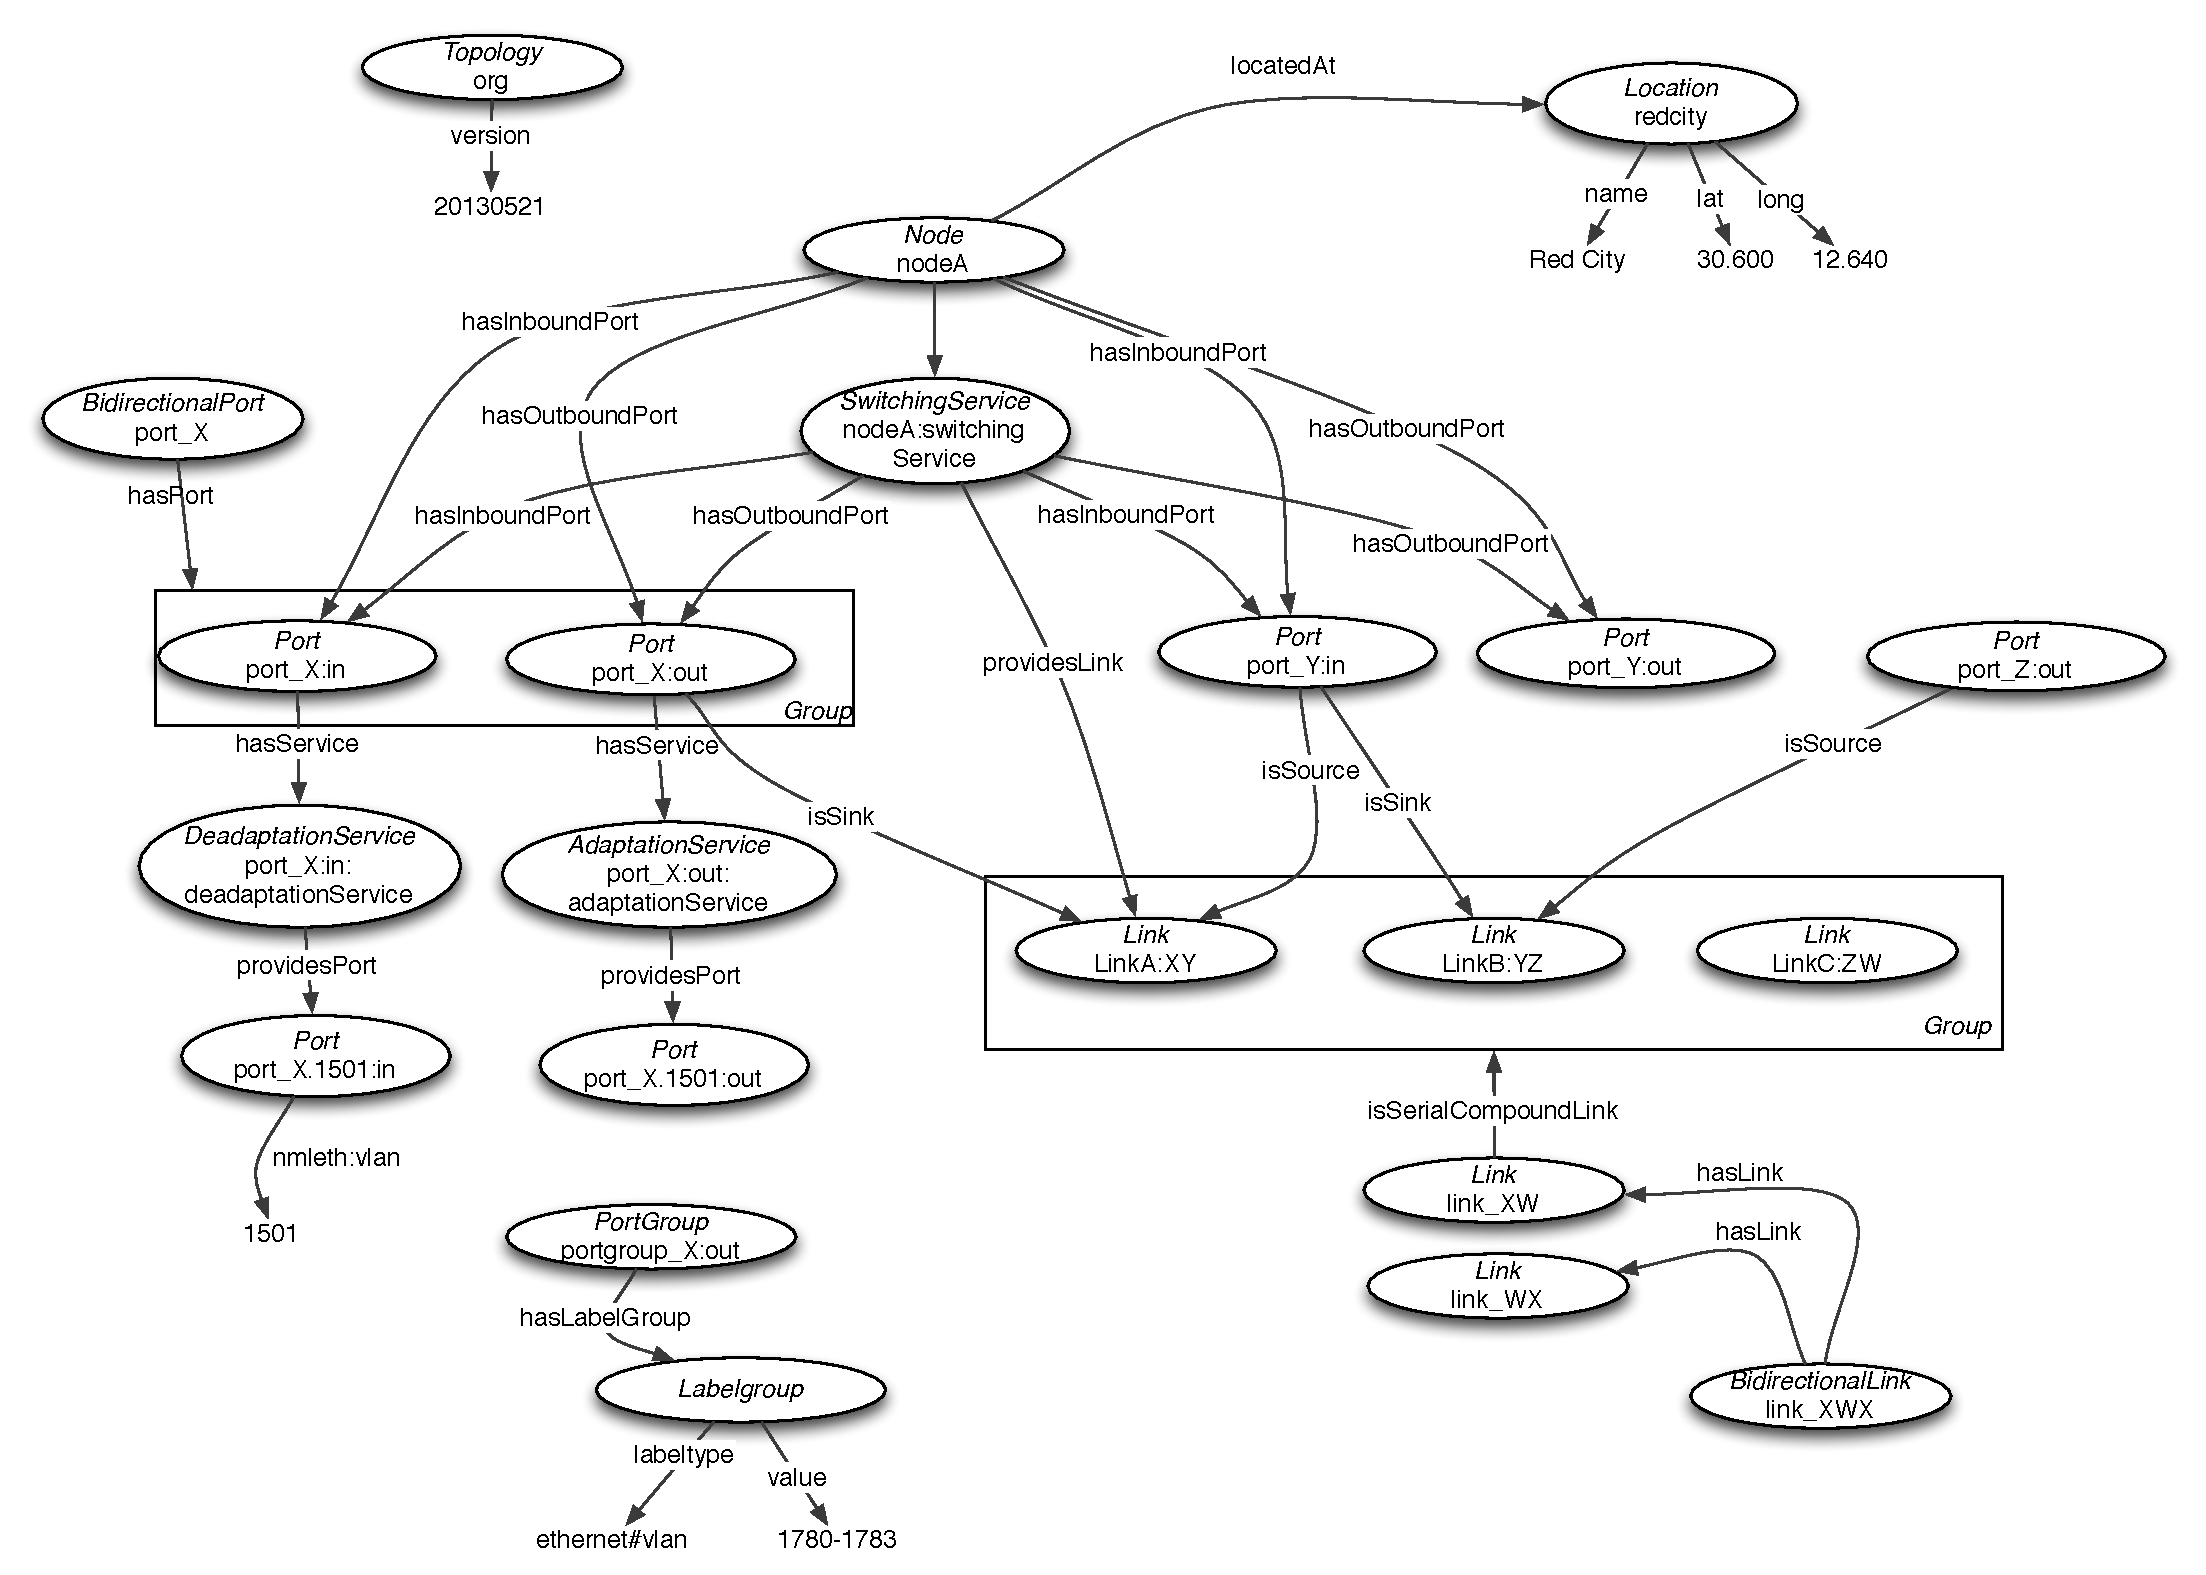
\includegraphics[width=\textwidth,angle=90]{combined-examples.pdf}
    \caption{A graphical overview showing the combination of all examples}
    \label{fig:combined-examples}
\end{figure}

\subsection{Examples in XML}
The following snippets represent NML structures in the XML format.

\begin{itemize}

    \item \emph{Topology} (section~\ref{class:topology})
      \lstinputlisting{xml/example-topology.xml}
    \item \emph{Node} (section~\ref{class:node})
      \lstinputlisting{xml/example-node.xml}
    \item \emph{Ports}  
      \begin{itemize}
        \item \emph{(Unidirectional) Port}  (section~\ref{class:port})
          \lstinputlisting{xml/example-port-unidir.xml}
        \item \emph{BidirectionalPort} (section~\ref{class:bidirectional_port})
          \lstinputlisting{xml/example-port-bidir.xml}
        \item \emph{PortGroup} (section~\ref{class:port_group})
          \lstinputlisting{xml/example-portgroup.xml}
      \end{itemize}
    \item \emph{Links} 
      \begin{itemize}
        \item \emph{UnidirectionalLink} (external) (section~\ref{class:link})
          \lstinputlisting{xml/example-link-unidir.xml}
        \item \emph{UnidirectionalLink} (internal) (section~\ref{class:link})
          \lstinputlisting{xml/example-link-unidir-cc.xml}
        \item \emph{UnidirectionalLink that is composed of more than one sub-link}
          \lstinputlisting{xml/example-link-serialcompound.xml}
        \item \emph{BidirectionalLink} (section~\ref{class:bidirectional_link})
          \lstinputlisting{xml/example-link-bidir.xml}
        \item \emph{LinkGroup} (section~\ref{class:link_group})
          \lstinputlisting{xml/example-linkgroup.xml}
      \end{itemize}
    \item \emph{Labels}
      \begin{itemize}
        \item \emph{Label} (section~\ref{class:label})
          \lstinputlisting{xml/example-label.xml}
        \item \emph{LabelGroup} (section~\ref{class:label_group})
          \lstinputlisting{xml/example-labelgroup.xml}
      \end{itemize}
    \item \emph{Location} (section~\ref{class:location})
      \lstinputlisting{xml/example-location.xml}
    \item \emph{Services}
      \begin{itemize}
        \item \emph{SwitchingService} (section~\ref{class:switching_service})
          \lstinputlisting{xml/example-switchingservice.xml}
        \item \emph{AdaptationService} (section~\ref{class:adaptation_service})
          \lstinputlisting{xml/example-adaptationservice.xml}
        \item \emph{DeadaptationService} (section~\ref{class:deadaptation_service})
          \lstinputlisting{xml/example-deadaptationservice.xml}
      \end{itemize}

\end{itemize}

\pagebreak

\subsection{Examples in OWL}
The following snippets represent NML structures in the OWL format.
The namespaces used in all the examples follow the definitions of the Topology example.

\begin{itemize}

    \item \emph{Topology} (section~\ref{class:topology})
      \lstinputlisting{owl/example-topology.xml}
    \item \emph{Node} (section~\ref{class:node})
      \lstinputlisting{owl/example-node.xml}
    \item \emph{Ports}  
      \begin{itemize}
        \item \emph{(Unidirectional) Port}  (section~\ref{class:port})
          \lstinputlisting{owl/example-port-unidir.xml}
        \item \emph{BidirectionalPort} (section~\ref{class:bidirectional_port})
          \lstinputlisting{owl/example-port-bidir.xml}
        \item \emph{PortGroup} (section~\ref{class:port_group})
          \lstinputlisting{owl/example-portgroup.xml}
      \end{itemize}
    \item \emph{Links} 
      \begin{itemize}
        \item \emph{UnidirectionalLink} (external) (section~\ref{class:link})
          \lstinputlisting{owl/example-link-unidir.xml}
        \item \emph{UnidirectionalLink} (internal) (section~\ref{class:link})
          \lstinputlisting{owl/example-link-unidir-cc.xml}
        \item \emph{UnidirectionalLink that is composed of more than one sub-link}
          \lstinputlisting{owl/example-link-serialcompound.xml}
        \item \emph{BidirectionalLink} (section~\ref{class:bidirectional_link})
          \lstinputlisting{owl/example-link-bidir.xml}
        \item \emph{LinkGroup} (section~\ref{class:link_group})
          \lstinputlisting{owl/example-linkgroup.xml}
      \end{itemize}
    \item \emph{Labels}
      \begin{itemize}
        \item \emph{Label} (section~\ref{class:label})
          \lstinputlisting{owl/example-label.xml}
        \item \emph{LabelGroup} (section~\ref{class:label_group})
          \lstinputlisting{owl/example-labelgroup.xml}
      \end{itemize}
    \item \emph{Location} (section~\ref{class:location})
      \lstinputlisting{owl/example-location.xml}
    \item \emph{Services}
      \begin{itemize}
        \item \emph{SwitchingService} (section~\ref{class:switching_service})
          \lstinputlisting{owl/example-switchingservice.xml}
        \item \emph{AdaptationService} (section~\ref{class:adaptation_service})
          \lstinputlisting{owl/example-adaptationservice.xml}
        \item \emph{DeadaptationService} (section~\ref{class:deadaptation_service})
          \lstinputlisting{owl/example-deadaptationservice.xml}
      \end{itemize}

\end{itemize}

\subsection{Conceptual Examples}

This section shows a few examples how NML was designed to be used. Like the other examples, this section is informative.  It may be possible that there are other ways to use the NML objects and attributes.

\subsubsection{Topology and Node}

A \emph{Topology} and \emph{Node} behave similar: they both contain inbound ports and outbound ports, and can contain a \emph{SwitchingService} to allow creation of internal links (cross connects) from inbound ports to outbound ports. Especially with the ability to create logical, sliced or virtual devices, the distinction is getting blurred.

The distinction is that a \emph{Node} is located at a single geographic location, while a \emph{Topology} is a set of geographically disperse Network Objects.

\subsubsection{Hierarchical Topology}

Large networks may want to publish both details of their network topology as a whole, as well as details about regional segments, without publishing details of the actual devices. NML allows the publication of a hierarchical \emph{Topology} tree, where the top-level \emph{Topology} has a \emph{hasTopology} relation with smaller \emph{Topologies}. These smaller Topologies must be fully enclosed -- the \emph{hasTopology} relation can not be used to relate partial overlapping Topologies.

For example, a \emph{Topology} \texttt{A} may want to publish about two parts of its Topology, \texttt{A\_West}, and \texttt{A\_East}. This allows it to publish difference in connectivity and costs between the two parts. It can do so with the following relations:

\nmlrelation{Topology \texttt{A}}{}{hasTopology}{}{Topology \texttt{A\_West}}\\
\nmlrelation{Topology \texttt{A}}{}{hasTopology}{}{Topology \texttt{A\_East}}

\subsubsection{Links, Segments and Paths}

A \emph{Link} object can refer to any link connection. A link segment and an end-to-end path are both described by a \emph{Link} object. This is by design, since it is easy to extend a \emph{Link}, or to describe a partition of a \emph{Link}.

Figure~\ref{fig:compound-link} gives an example of three different partitionings of a link between \texttt{port\_X:in} and \texttt{port\_W:out}.

\begin{figure}[htb]
    \centering
        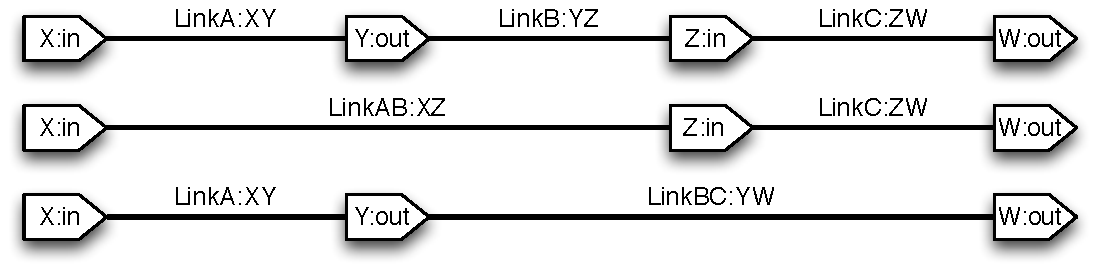
\includegraphics[width=.8\textwidth]{compound-link.pdf}
    \caption{Different partitionings of the same link.}
    \label{fig:compound-link}
\end{figure}

Note that in this example Port \texttt{port\_Y:out} is the source of both \texttt{linkB:YZ} and of \texttt{linkBC:YW}. If a single topology description would contain the full link and the partitioning, a path finding algoritm \MUST{} be aware that the fact that if a Port is the source of two NML Links, this does not mean it multicast to different network links. For this reason, it is \RECOMMENDED{} that applications either add metadata about the type of link, or specify that in certain messages, only one particular type of Link \MUST{} be used.


\subsubsection{Patch Panel and Media Convertor}

A port on a patch panel or optical distribution frame can simply be described as a NML Port (thus without an associated Node):

\nmlrelation{Port \texttt{odf\_X}}{}{isSink}{}{Link \texttt{A}}\\
\nmlrelation{Port \texttt{odf\_X}}{}{isSource}{}{Link \texttt{B}}

A mediaconvertor, e.g. from Ethernet over UTP to Ethernet over fiber, can be described in the same way, provided that the connected Links described the Ethernet connections. If the connected Links describe the underlying UTP and fiber connections, it is necessary to describe the conversion between them:

\nmlrelation{Port \texttt{Port\_X\_UTP}}{}{isSink}{}{Link \texttt{UTP\_A}} \\
\nmlrelation{Port \texttt{Port\_X\_fiber}}{}{isSource}{}{Link \texttt{fiber\_B}} \\
\nmlrelation{Port \texttt{Port\_X\_UTP}}{}{hasService}{}{DeAdaptataionService \texttt{X\_deadaptation}} \\
\nmlrelation{Port \texttt{Port\_X\_fiber}}{}{hasService}{}{AdaptationService \texttt{X\_adaptation}} \\
\nmlrelation{DeAdaptataionService \texttt{X\_deadaptation}}{}{providesPort}{}{Port \texttt{Port\_X\_eth}} \\
\nmlrelation{AdaptationService \texttt{X\_adaptation}}{}{providesPort}{}{Port \texttt{Port\_X\_eth}}


\subsubsection{VLAN and Broadcast Medium}

A VLAN is much like a broadcast medium, which can be described as a multipoint-to-multipoint Link:

\nmlrelation{Port \texttt{Port\_X:in}}{}{isSink}{}{Link \texttt{VLAN\_42}} \\
\nmlrelation{Port \texttt{Port\_X:out}}{}{isSink}{}{Link \texttt{VLAN\_42}} \\
\nmlrelation{Port \texttt{Port\_Y:in}}{}{isSink}{}{Link \texttt{VLAN\_42}} \\
\nmlrelation{Port \texttt{Port\_Y:out}}{}{isSink}{}{Link \texttt{VLAN\_42}} \\
\nmlrelation{Port \texttt{Port\_Z:in}}{}{isSink}{}{Link \texttt{VLAN\_42}} \\
\nmlrelation{Port \texttt{Port\_Z:out}}{}{isSink}{}{Link \texttt{VLAN\_42}} \\

Where \texttt{X}, \texttt{Y} and \texttt{Z} are in fact bidirectional ports:

\nmlrelation{BidirectionalPort \texttt{Port\_X}}{}{hasPort}{}{Port \texttt{Port\_X:in}} \\
\nmlrelation{BidirectionalPort \texttt{Port\_X}}{}{hasPort}{}{Port \texttt{Port\_X:out}} \\
\nmlrelation{BidirectionalPort \texttt{Port\_Y}}{}{hasPort}{}{Port \texttt{Port\_Y:in}} \\
\nmlrelation{BidirectionalPort \texttt{Port\_Y}}{}{hasPort}{}{Port \texttt{Port\_Y:out}} \\
\nmlrelation{BidirectionalPort \texttt{Port\_Z}}{}{hasPort}{}{Port \texttt{Port\_Z:in}} \\
\nmlrelation{BidirectionalPort \texttt{Port\_Z}}{}{hasPort}{}{Port \texttt{Port\_Z:out}} \\

However, this is not entirely correct: in the above description data coming from \texttt{Port\_X:in} would also be forwarded to \texttt{Port\_X:out}. However, the Ethernet technology prevents data returning on the same interface.

NML introduced the \emph{noReturnTraffic} parameter to describe this technological restriction: if the \emph{noReturnTraffic} parameter of a Link is true, there is no data transport from a source to a sink if the source and sink are grouped together in a BidirectionalPort group.

\nmlrelation{Link VLAN\_42}{}{noReturnTraffic}{}{"\texttt{true}"} \\


\subsubsection{Configuration and Potential Capability}

NML is able to both describe the network services (potential capability) as well as the network configuration.

A switching service can be described by a SwitchingService object along with associated inbound ports and outbound ports:

\nmlrelation{SwitchingService \texttt{switchmatrix\_A}}{}{hasInboundPort}{}{PortGroup \texttt{Port\_X:in}} \\
\nmlrelation{SwitchingService \texttt{switchmatrix\_A}}{}{hasOutboundPort}{}{PortGroup \texttt{Port\_X:out}} \\
\nmlrelation{SwitchingService \texttt{switchmatrix\_A}}{}{hasInboundPort}{}{PortGroup \texttt{Port\_Y:in}} \\
\nmlrelation{SwitchingService \texttt{switchmatrix\_A}}{}{hasOutboundPort}{}{PortGroup \texttt{Port\_Y:out}} \\
\nmlrelation{SwitchingService \texttt{switchmatrix\_A}}{}{labelSwapping}{}{\texttt{true}}

A cross connect created by this switching service can be specified by a Link object:

\nmlrelation{SwitchingService \texttt{switchmatrix\_A}}{}{providesLink}{}{Link \texttt{crossconnect\_A.1501}} \\
\nmlrelation{PortGroup \texttt{Port\_X:in}}{}{hasPort}{}{Port \texttt{Port\_X.1501:in}} \\
\nmlrelation{PortGroup \texttt{Port\_Y:out}}{}{hasPort}{}{Port \texttt{Port\_Y.1501:out}} \\
\nmlrelation{Port \texttt{Port\_X.1501:in}}{}{isSource}{}{Link \texttt{crossconnect\_A.1501}} \\
\nmlrelation{Port \texttt{Port\_Y.1501:out}}{}{isSink}{}{Link \texttt{crossconnect\_A.1501}}

An encoding and decoding service can be described by a AdapdationService and DeAdaptationService:

\nmlrelation{Port \texttt{Port\_X\_fiber:in}}{}{hasService}{}{DeAdaptationService \texttt{port\_X:in:deadaptation}} \\
\nmlrelation{DeAdaptationService \texttt{port\_X:in:deadaptation}}{}{canProvidePort}{}{PortGroup \texttt{Port\_X:in}}

A channel created by this encoding service can be specified by a \emph{providesPort} relation:

\nmlrelation{DeAdaptationService \texttt{port\_X:in:deadaptation}}{}{providesPort}{}{Port \texttt{Port\_X.1501:in}} \\
\nmlrelation{PortGroup \texttt{Port\_X:in}}{}{hasPort}{}{Port \texttt{Port\_X.1501:in}}


\subsubsection{Versioning and Lifetime}

The version of a \emph{Topology} indicated the serial number. If there are two \emph{Topology} descriptions for the same network, the one with the highest version number is the most recent version. The \emph{LifeTime} object is used to indicate when a certain resource is available.

Imagine that a link will have a scheduled downtime due to maintenance next week between 2 AM and 4 AM. This can be specified with these relations:

\nmlrelation{Topology \texttt{org}}{}{version}{}{\texttt{20130521T000000Z}} \\
\nmlrelation{Link \texttt{A}}{}{existsDuring}{}{LifeTime \texttt{A\_lifetime1}} \\
\nmlrelation{Link \texttt{A}}{}{existsDuring}{}{LifeTime \texttt{A\_lifetime2}} \\
\nmlrelation{LifeTime \texttt{A\_lifetime1}}{}{end}{}{\texttt{20130611T020000Z}} \\
\nmlrelation{LifeTime \texttt{A\_lifetime2}}{}{start}{}{\texttt{20130611T040000Z}}

Imagine that this planned maintainance is rescheduled. That can be specified by creating a new Topology with a new version number, and updated data:

\nmlrelation{Topology \texttt{org}}{}{version}{}{\texttt{20130604T000000Z}} \\
\nmlrelation{Link \texttt{A}}{}{existsDuring}{}{LifeTime \texttt{A\_lifetime1}} \\
\nmlrelation{Link \texttt{A}}{}{existsDuring}{}{LifeTime \texttt{A\_lifetime2}} \\
\nmlrelation{LifeTime \texttt{A\_lifetime1}}{}{end}{}{\texttt{20130618T020000Z}} \\
\nmlrelation{LifeTime \texttt{A\_lifetime2}}{}{start}{}{\texttt{20130618T040000Z}}



%!TEX root = nml-base.tex

\section{Security Considerations}%
\label{s:security}

% Please refer to RFC 3552~\cite{rfc3552} for guidance on writing a security considerations section.  This section is required in all documents, and should not just say ``there are no security considerations.''  Quoting from the RFC: 
% 
% \begin{quote}
% ``Most people speak of security as if it were a single monolithic property of a protocol or system, however, upon reflection, one realizes that it is clearly not true.  Rather, security is a series of related but somewhat independent properties.  Not all of these properties are required for every application.
% 
% We can loosely divide security goals into those related to protecting communications (COMMUNICATION SECURITY, also known as COMSEC) and those relating to protecting systems (ADMINISTRATIVE SECURITY or SYSTEM SECURITY).  Since communications are carried out by systems and access to systems is through communications channels, these goals obviously interlock, but they can also be independently provided.''
% \end{quote}

There are important security concerns associated with the generation and distribution of network topology information. For example, ISPs frequently consider network topologies to be confidential. We do not address these concerns in this document, but implementers are encouraged to consider the security implications of generating and distributing network topology information. 

Implementers should be aware that the NML descriptions do not provide any guarantee regarding their integrity nor their authenticity. The NML documents also can not provide this for the identifiers contained in the documents. Implementers should use external means of verifying the authenticity of identifiers contained in the documents.
% 
\section{Glossary}
\label{s:glossary}

\begin{description}
\item[metric] a metric is a mathematical representation of a well defined aspect of a physical entity
\item[measurement] a measurement is the process of extracting a metric from a physical entity, and by extension also the result of such process. The measurement seldom corresponds exactly to the value of the metric.
\item[SLA] {\em ``An agreement defines a dynamically-established and dynamically
managed relationship between parties. The object of this
relationship is the delivery of a service by one of the parties within
the context of the agreement.''} from {\em SLA@SOI Glossary}
\item[Restful model] {\em ``REST is a coordinated set of architectural constraints that attempts to minimize latency and network communication, while at the same time maximizing
the independence and scalability of component implementations.''} \cite{fie02a}
\item[OCCI] {``\em The Open Cloud Computing Interface (OCCI) is a RESTful Protocol and API for all kinds of management tasks. OCCI was originally initiated to create a remote management API for IaaS model-based services, allowing for the development of interoperable tools for common tasks including deployment, autonomic scaling and monitoring''} \cite{occi:core}
\item[OCCI {\em Kind}] {\em''The Kind type represents the type identification mechanism for all Entity types present in the model''} \cite{occi:core}
\item[OCCI {\em \ln}] {\em''An instance of the Link type defines a base association between two Resource instances.''} \cite{occi:core}
\item[OCCI \mi] {\em''The Mixin type represent an extension mechanism, which allows new resource
capabilities to be added to resource instances both at creation-time and/or run-time.''} \cite{occi:core}
\item[OCCI \rs] {\em''A Resource is suitable to represent real world resources, e.g. virtual machines, networks, services, etc. through specialisation.''} \cite{occi:core}
\item[\sens] The \sens\ is a \rs\ that collects metrics from its input side, and delivers aggregated metrics from its output
\item[\coll] The \coll\ is a link that conveys metrics: it defines both the transport protocol and the conveyed metrics.
\end{description}


\section{Contributors}

% Contact information for authors. You can also use this section to recognize contributions by other people who are not listed as authors, but made a useful contribution.
% 
% The title page should list the Corresponding Authors (or Editors), who are committed to taking permanent stewardship for this document – receiving communication in the future and otherwise being responsive to its content. Corresponding authors will be sought to process any error reports. The title page should contain at least one and at most three (Corresponding) Author/Editors, unless there are compelling reasons to list more.
% 
% Corresponding authors must be indicated as part of the Contributors or Authors section. Contributors are individuals who assisted with a document's preparation, and whose contributions are recognized in the document.
% 
% The OGF prefers the use of full first names (not initials). Complete contact information for authors must be included. Contributors are listed after authors, and do not need to have complete contact information. The nature of the contribution may be recognized.

\textbf{Jeroen J. van der Ham (Editor)} \\
Faculty of Science, Informatics Institute, University of Amsterdam \\
Science Park 904, 1098 XH  Amsterdam  \\
The Netherlands \\
Email: vdham@uva.nl \\
\\
\textbf{Freek Dijkstra} \\
SURFsara \\
Science Park 140,  1098 XG  Amsterdam \\
The Netherlands \\
Email: freek.dijkstra@surfsara.nl \\
\\
\textbf{Roman Łapacz} \\
PSNC \\
ul. Noskowskiego 12/14,  61-704 Poznań \\
Poland \\
Email: romradz@man.poznan.pl \\
\\
\textbf{Jason Zurawski} \\
Internet2 \\
1150 18th Street, NW \\
Suite 900 \\
Washington, DC 20036 \\
USA \\
Email: zurawski@es.net % \\


\section{Acknowledgments}

The authors would like to thank the NML working group members for their patience.
The NML group has operated in the web of infrastructure groups and is grateful for all the input from the NM, NMC and NSI working-groups.

Financial support has been provided by several projects and institutions: 

This work was partially supported by the European Commission, $7^{th}$ Framework Programme for Research and Technological Development, Capacities,  The GN3 project -- Grant No. 238875, GEYSERS -- Grant No. 248657 and NOVI -- Grant No. 257867.
This project was also made possible by the support of SURF, the collaborative organisation for higher education institutes and research institutes aimed at breakthrough innovations in ICT. More information on SURF is available on the website www.surf.nl.
Furthermore, this work was supported by the Dutch national program COMMIT.

Jason Zurawski would like to thank Internet2, along with the National Science Foundation (NSF) for support through grants: \#0962704, \#1019008, and \#0721902.

The authors are indebted to the many participants of working group sessions and on the mailing list, including the following contributors: 
Aaron Brown,
Jeff W. Boote, 
Aur\'elien Cedeyn, 
Evangelos Chaniotakis, 
Chin Guok, 
Paola Grosso, 
Richard Hughes-Jones, 
Houssem Medhioub, 
Ralph Niederberger, 
Anand Patil, 
Victor Reijs, 
Guy Roberts, 
Jerry Sobieski, 
Martin Swany, 
Fausto Vetter, 
Pascale Vicat-Blanc, and
John Vollbrecht.


%!TEX root = nml-base.tex

\section{Intellectual Property Statement}

The OGF takes no position regarding the validity or scope of any intellectual property or other rights that might be claimed to pertain to the implementation or use of the technology described in this document or the extent to which any license under such rights might or might not be available; neither does it represent that it has made any effort to identify any such rights.  Copies of claims of rights made available for publication and any assurances of licenses to be made available, or the result of an attempt made to obtain a general license or permission for the use of such proprietary rights by implementers or users of this specification can be obtained from the OGF Secretariat.

The OGF invites any interested party to bring to its attention any copyrights, patents or patent applications, or other proprietary rights which may cover technology that may be required to practice this recommendation.  Please address the information to the OGF Executive Director.

\section{Disclaimer}

This document and the information contained herein is provided on an ``As Is'' basis and the OGF disclaims all warranties, express or implied, including but not limited to any warranty that the use of the information herein will not infringe any rights or any implied warranties of merchantability or fitness for a particular purpose.

\section{Full Copyright Notice}

Copyright \copyright \ Open Grid Forum (\copyrightyears). Some Rights Reserved.

This document and translations of it may be copied and furnished to
others, and derivative works that comment on or otherwise explain it
or assist in its implementation may be prepared, copied, published and
distributed, in whole or in part, without restriction of any kind,
provided that the above copyright notice and this paragraph are
included as references to the derived portions on all such copies and
derivative works. The published OGF document from which such works are
derived, however, may not be modified in any way, such as by removing
the copyright notice or references to the OGF or other organizations,
except as needed for the purpose of developing new or updated OGF
documents in conformance with the procedures defined in the OGF
Document Process, or as required to translate it into languages other
than English. OGF, with the approval of its board, may remove this
restriction for inclusion of OGF document content for the purpose of
producing standards in cooperation with other international standards
bodies.

The limited permissions granted above are perpetual and will not be
revoked by the OGF or its successors or assignees. 

\begin{appendices}
	%!TEX root = nml-base.tex

\section{XML Schema}%
\label{app:xml}

This section describes the normative schema of XML documents using the XML Schema language.

\lstinputlisting{schemas/nsi-ext.xsd}
	%!TEX root = nml-base.tex

\section{OWL Schema}%
\label{s:owlschema}

This section describes the normative schema of the OWL syntax using the OWL ontology definition below.


% This section describes the normative schema of the OWL syntax using the following OWL ontology. First is the OWL syntax used for the RDF/XML notation, and we also include the Notation3 version of the ontology.
% 
% \subsection{OWL RDF/XML Schema} % (fold)
% \label{sub:owl_rdf_xml_schema}

\lstinputlisting{schemas/nml-base.owl}
% subsection owl_rdf_xml_schema (end)

% \subsection{OWL Notation3 Schema} % (fold)
% \label{sub:owl_notation3_schema}
% 
% \lstinputlisting{schemas/nml-base.n3}
% subsection owl_notation3_schema (end)

	%!TEX root = nml-base.tex

\section{Relation to G.800}%
\label{s:g800terms}

This section describes the relation between terms defined in this recommendation and those defined in the ITU-T G.800 recommendation~\cite{g800}.

\begin{tabular}{ll}
\hline
\textbf{NML Term} & \textbf{G.800 Term}\\
\hline
Port & Unidirectional Port \\
\hline
Link & Either Link Connection or Network Connection \\
\hline
SwitchingService & Subnetwork \\
\hline
AdaptationService & Combined Adaptation Function and Termination Function \\
\hline
BidirectionalPort & Port \\
\hline
Label & Resource label \\
\hline
\end{tabular}

\end{appendices}

%!TEX root = nml-base.tex
\phantomsection\addcontentsline{toc}{section}{References}%
\section*{References}%
\label{s:references}
% 
% Define heading of bibliography to be empty, since we already have a heading above the text.
\renewcommand{\refname}{}

\phantomsection\addcontentsline{toc}{subsection}{Normative References}
\subsection*{Normative References}
\begin{thebibliography}{10}
\vspace*{-3em}

\bibitem[GFD.202]{gfd.202}
Freek Dijkstra, and Jeroen van der Ham.
\newblock {A URN Namespace for Network Resources}.
\newblock GFD 202 (Community Practise), June 2013.
\newblock URL \url{http://www.ogf.org/documents/GFD.202.pdf}.

\bibitem[ISO 8601]{iso8601}
% No author
\newblock {Data elements and interchange formats -- Information interchange -- Representation of dates and times}.
\newblock ISO 8601:2004 (Third edition), December 2004.
\newblock Section 4.3.2 (a), Complete representations of a date and time. Calendar date in basic format.
\newblock URL \url{http://www.iso.org/iso/home/store/catalogue_ics/catalogue_detail_ics.htm?csnumber=40874}.

\bibitem[G.800]{g800}
% No author
\newblock {Unified functional architecture of transport networks}.
\newblock ITU-T Recommendation G.800, February 2012.
\newblock URL \url{http://www.itu.int/rec/T-REC-G.800/}.

\bibitem[RDF-XML]{rdfxml}
Dave Beckett (editor)
\newblock {RDF/XML Syntax Specification (Revised)}
\newblock {W3C Recommendation 10 February 2004}.
\newblock URL \url{http://www.w3.org/TR/rdf-syntax-grammar/}.

\bibitem[RFC 2119]{rfc2119}
Scott Bradner.
\newblock {Key words for use in RFCs to Indicate Requirement Levels}.
\newblock RFC 2119 (Best Current Practice), March 1997.
\newblock URL \url{http://tools.ietf.org/html/rfc2119}.

\bibitem[RFC 3492]{punycode}
A. Costello
\newblock {Punycode: A Bootstring encoding of Unicode for Internationalized Domain Names in Applications (IDNA)}
\newblock RFC 3492 (Standards Track), March 2003
\newblock URL \url{http://tools.ietf.org/html/rfc3492}.

\bibitem[RFC 3986]{rfc3986}
Tim Berners-Lee, Roy T. Fielding, and Larry Masinter.
\newblock {Uniform Resource Identifier (URI): Generic Syntax}
\newblock RFC 3986 (Standards Track), January 2005.
\newblock URL \url{http://tools.ietf.org/html/rfc3986}.

\bibitem[Unicode]{casefolding}
The Unicode Consortium.
\newblock The Unicode Standard, Version 6.2.0. 
\newblock Mountain View, CA, USA. November 2012. ISBN 978-1-936213-07-8
\newblock Section 5.18, Case Mappings. Paragraph about Caseless Matching.
\newblock Normative URL \url{http://www.unicode.org/versions/Unicode6.2.0/}
\newblock Informative URL \url{ftp://ftp.unicode.org/Public/UNIDATA/CaseFolding.txt}

\bibitem[UNLOCODE]{unlocode}
% No author
\newblock {United Nations Code for Trade and Transport Locations}
\newblock UN/LOCODE, revision 2012-01, September 2012.
\newblock URL \url{http://www.unece.org/cefact/locode/welcome.html}.

\bibitem[WGS84]{wgs84}
% No author
\newblock {Department of Defense World Geodetic System 1984, Its Definition and Relationships With Local Geodetic Systems}
\newblock NIMA Technical Report TR8350.2, Third Edition, June 2004
\newblock URL \url{http://earth-info.nga.mil/GandG/publications/tr8350.2/tr8350_2.html}.

\bibitem[XML]{xml}
Henry S. Thompson, David Beech, Murray Maloney and Noah Mendelsohn
\newblock {XML Schema Part 1: Structures Second Edition}
\newblock {W3C Recommendation 28 October 2004}.
\newblock URL \url{http://www.w3.org/TR/xmlschema-1/}.

\end{thebibliography}

\phantomsection\addcontentsline{toc}{subsection}{Informative References}
\subsection*{Informative References}

\begin{thebibliography}{10}
\vspace*{-3em}

\bibitem[Dijkstra13]{nml-experimental}
Freek Dijkstra, et al.
\newblock {Experimental Features for NML 1}.
\newblock Work in Progress.

\bibitem[GFD.165]{gfd.165}
Paola Grosso, Aaron Brown, Aur\'elien Cedeyn, Freek Dijkstra, Jeroen van der Ham, Anand Patil, Pascale Primet, Martin Swany, and Jason Zurawski.
\newblock {Network Topology Descriptions in Hybrid Networks}
\newblock GFD 165 (Informational), March 2010.
\newblock URL \url{http://www.ogf.org/documents/GFD.165.pdf}.

\bibitem[RFC 6350]{vcard}
Simon Perreault.
\newblock {vCard Format Specification}
\newblock RFC 6350 (Standards Track), August 2011.
\newblock URL \url{http://tools.ietf.org/html/rfc6350}.

\bibitem[RFC 6351]{xcard}
S. Perreault.
\newblock {xCard: vCard XML Representation}
\newblock RFC 6351 (Standards Track), August 2011.
\newblock URL \url{http://tools.ietf.org/html/rfc6351}.

\bibitem[RDFVCARD]{rdf-vcard}
 Harry Halpin, Renato Iannella, Brian Suda, Norman Walsh
\newblock Representing vCard Objects in RDF
\newblock W3C Member Submission 20 January 2010.
\newblock URL \url{http://www.w3.org/TR/vcard-rdf/}.


\end{thebibliography}
 

\end{document}
